\chapter{Appendix}\label{ch:appendix}

\section{Property Graph Schema: Full Cypher Constraints}
\label{sec:appendix-schema}

The following Cypher statements create the uniqueness constraints and
indexes used by the pipeline, using the actual node labels from
\cref{tab:node-types}.

\begin{minted}{cypher}
// Uniqueness constraints
CREATE CONSTRAINT fn_def_unique IF NOT EXISTS
  FOR (f:CppFunctionDefinition)
  REQUIRE f.qualified_name IS UNIQUE;

CREATE CONSTRAINT fn_decl_unique IF NOT EXISTS
  FOR (f:CppFunctionDeclaration)
  REQUIRE f.qualified_name IS UNIQUE;

CREATE CONSTRAINT decl_unique IF NOT EXISTS
  FOR (d:CppDeclaration)
  REQUIRE d.qualified_name IS UNIQUE;

CREATE CONSTRAINT symbol_unique IF NOT EXISTS
  FOR (s:Symbol) REQUIRE s.name IS UNIQUE;

// Indexes for lookup performance
CREATE INDEX fn_source IF NOT EXISTS
  FOR (f:CppFunctionDefinition) ON (f.source_file, f.line);

CREATE INDEX file_path IF NOT EXISTS
  FOR (f:SourceFile) ON (f.path);
\end{minted}

\section{csp\_matcher Tracing Rules for CPSCore}
\label{sec:appendix-tracing-rules}

The following rules file (\texttt{add\_tracing.txt}) specifies the three
call-site patterns instrumented by \texttt{csp\_matcher} during trace
collection (\cref{sec:csp-matcher}).
Each \texttt{find:}/\texttt{replace:} pair wraps a target call expression
with a comma-operator trace emission that captures caller context at the
call site.

\begin{minted}[fontsize=\footnotesize]{text}
find:    $agg.getAll<$T>()
replace: (std::fprintf(stderr,
           "[TRACE] %s, $callerFunc, %s, Aggregator.getAll,
            Aggregation, $callerClass, %s\n",
           cspTraceTimestamp().c_str(),
           cspTraceCallerComponent(__FILE__).c_str(),
           cspTraceLocation(__FILE__, __LINE__).c_str()),
          $agg.getAll<$T>())

find:    CPSLogger::instance()->flush()
replace: (std::fprintf(stderr,
           "[TRACE] %s, $callerFunc, %s, CPSLogger.flush,
            Logging, $callerClass, %s\n",
           cspTraceTimestamp().c_str(),
           cspTraceCallerComponent(__FILE__).c_str(),
           cspTraceLocation(__FILE__, __LINE__).c_str()),
          CPSLogger::instance()->flush())

find:    EnumMap<RunStage>::convert($stage)
replace: (std::fprintf(stderr,
           "[TRACE] %s, $callerFunc, %s, EnumMap.convert,
            Utilities, $callerClass, %s\n",
           cspTraceTimestamp().c_str(),
           cspTraceCallerComponent(__FILE__).c_str(),
           cspTraceLocation(__FILE__, __LINE__).c_str()),
          EnumMap<RunStage>::convert($stage))
\end{minted}

The corresponding removal rule (\texttt{remove\_tracing.txt}) uses a
filter function to identify and strip trace wrappers:

\begin{minted}[fontsize=\footnotesize]{text}
find:    ($any, $orig)
filter:  is_trace_remove
replace: $orig
\end{minted}

The filter (\texttt{tracing\_filters.cpp}) accepts only comma expressions
whose left operand contains the \texttt{[TRACE]} marker:

\begin{minted}[fontsize=\footnotesize]{cpp}
bool is_trace_remove(int n, const char* const* ns,
                     const char* const* vs) {
    const char* text = get_hole(n, ns, vs, "any");
    return text != NULL && strstr(text, "[TRACE]") != NULL;
}
\end{minted}

This ensures that only trace-injected comma expressions are removed,
leaving any pre-existing comma expressions in the codebase untouched.

\section{Ground-Truth Reference Diagrams (S1--S3)}
\label{sec:appendix-groundtruth}

The manually authored \sysml reference diagrams used as ground truth for
the H1 evaluation (\cref{sec:h1-results}).
Each pair consists of a structural diagram (component connectivity) and a
sequence diagram (message interactions).

\subsection{S1: Aggregator Notification Chain, Structural}

\begin{minted}[fontsize=\footnotesize]{text}
package 'S1-Structural' {

    part def Synchronization {
        part aggregatableRunner : AggregatableRunner;
        part simpleRunner       : SimpleRunner;
        part synchronizedRunner : SynchronizedRunner;
        part syncRunnerMaster   : SynchronizedRunnerMaster;
    }

    part def Aggregation {
        part aggregator : Aggregator;
    }

    part def Logging {
        part cpsLogger     : CPSLogger;
        part raiiLogStream : RAIILogStream;
    }

    interface def IAggregator {
        in  feature request  : 'getAll';
        out feature response : 'ObjectList';
    }

    interface def ICPSLogger {
        in feature flush    : 'flush';
        in feature instance : 'instance';
    }

    interface def IRAIILogStream {
        in feature stream : 'stream';
    }

    connection : IAggregator
        connect Synchronization::aggregatableRunner to Aggregation::aggregator;
    connection : IAggregator
        connect Synchronization::simpleRunner       to Aggregation::aggregator;
    connection : IAggregator
        connect Synchronization::synchronizedRunner  to Aggregation::aggregator;

    connection : IRAIILogStream
        connect Synchronization::simpleRunner        to Logging::raiiLogStream;
    connection : IRAIILogStream
        connect Synchronization::syncRunnerMaster    to Logging::raiiLogStream;

    connection : ICPSLogger
        connect Synchronization::synchronizedRunner  to Logging::cpsLogger;
}
\end{minted}

\subsection{S1: Aggregator Notification Chain, Sequence}

\begin{minted}[fontsize=\footnotesize]{text}
package 'S1-Sequence' {

    part sync  : Synchronization;
    part agg   : Aggregation;
    part log   : Logging;

    message m1 from sync.syncRunnerMaster to log.raiiLogStream
        : 'RAIILogStream.stream';
    message m2 from sync.synchronizedRunner to agg.aggregator
        : 'Aggregator.getAll';
    message m3 from sync.synchronizedRunner to log.cpsLogger
        : 'CPSLogger.flush';
    message m4 from sync.synchronizedRunner to log.cpsLogger
        : 'CPSLogger.instance';
    message m5 from sync.aggregatableRunner to agg.aggregator
        : 'Aggregator.getAll';
    message m6 from sync.simpleRunner to agg.aggregator
        : 'Aggregator.getAll';
    message m7 from sync.simpleRunner to log.raiiLogStream
        : 'RAIILogStream.stream';
    message m8 from sync.simpleRunner to log.raiiLogStream
        : 'RAIILogStream.stream';
    message m9 from sync.simpleRunner to log.raiiLogStream
        : 'RAIILogStream.stream';
    message m10 from sync.syncRunnerMaster to log.raiiLogStream
        : 'RAIILogStream.stream';
    message m11 from sync.syncRunnerMaster to log.raiiLogStream
        : 'RAIILogStream.stream';
}
\end{minted}

\subsection{S2: Configuration Property Mapping, Structural}

\begin{minted}[fontsize=\footnotesize]{text}
package 'S2-Structural' {

    part def Configuration {
        part propertyMapper : PropertyMapper;
    }

    part def Logging {
        part raiiLogStream : RAIILogStream;
    }

    interface def IRAIILogStream {
        in feature stream : 'stream';
    }

    connection : IRAIILogStream
        connect Configuration::propertyMapper to Logging::raiiLogStream;
}
\end{minted}

\subsection{S2: Configuration Property Mapping, Sequence}

\begin{minted}[fontsize=\footnotesize]{text}
package 'S2-Sequence' {

    part cfg : Configuration;
    part log : Logging;

    message m1 from cfg.propertyMapper to log.raiiLogStream
        : 'RAIILogStream.stream';   // PropertyMapper.add
    message m2 from cfg.propertyMapper to log.raiiLogStream
        : 'RAIILogStream.stream';   // PropertyMapper.add (overload)
    message m3 from cfg.propertyMapper to log.raiiLogStream
        : 'RAIILogStream.stream';   // PropertyMapper.addEigen
    message m4 from cfg.propertyMapper to log.raiiLogStream
        : 'RAIILogStream.stream';   // PropertyMapper.addEnum
    message m5 from cfg.propertyMapper to log.raiiLogStream
        : 'RAIILogStream.stream';   // PropertyMapper.addVector
    message m6 from cfg.propertyMapper to log.raiiLogStream
        : 'RAIILogStream.stream';   // PropertyMapper.getChild
    message m7 from cfg.propertyMapper to log.raiiLogStream
        : 'RAIILogStream.stream';   // PropertyMapper.mandatoryCheck
}
\end{minted}

\subsection{S3: Multi-Component Runner Orchestration, Structural}

\begin{minted}[fontsize=\footnotesize]{text}
package 'S3-Structural' {

    part def Synchronization {
        part simpleRunner    : SimpleRunner;
        part syncMaster      : SynchronizedRunnerMaster;
    }

    part def Aggregation {
        part aggregator : Aggregator;
    }

    part def Utilities {
        part enumMap : EnumMap;
    }

    part def Logging {
        part raiiLogStream : RAIILogStream;
    }

    interface def IAggregator {
        in  feature request  : 'getAll';
        out feature response : 'ObjectList';
    }

    interface def IEnumMap {
        in  feature convert : 'convert';
        out feature label   : 'string';
    }

    interface def IRAIILogStream {
        in feature stream : 'stream';
    }

    connection : IAggregator
        connect Synchronization::simpleRunner to Aggregation::aggregator;
    connection : IEnumMap
        connect Synchronization::simpleRunner to Utilities::enumMap;
    connection : IRAIILogStream
        connect Synchronization::simpleRunner to Logging::raiiLogStream;
    connection : IRAIILogStream
        connect Synchronization::syncMaster to Logging::raiiLogStream;
}
\end{minted}

\subsection{S3: Multi-Component Runner Orchestration, Sequence}

\begin{minted}[fontsize=\footnotesize]{text}
package 'S3-Sequence' {

    part sync : Synchronization;
    part agg  : Aggregation;
    part util : Utilities;
    part log  : Logging;

    message m1 from sync.simpleRunner to agg.aggregator
        : 'Aggregator.getAll';
    message m2 from sync.simpleRunner to util.enumMap
        : 'EnumMap.convert';
    message m3 from sync.simpleRunner to log.raiiLogStream
        : 'RAIILogStream.stream';
    message m4 from sync.simpleRunner to util.enumMap
        : 'EnumMap.convert';
    message m5 from sync.simpleRunner to log.raiiLogStream
        : 'RAIILogStream.stream';
    message m6 from sync.syncMaster to log.raiiLogStream
        : 'RAIILogStream.stream';
}
\end{minted}

\section{Generated Pipeline Output (C5: Full Pipeline)}
\label{sec:appendix-generated}

The following shows representative output from the full pipeline condition
(C5: static + dynamic + scenario scoping, \cref{sec:h1-results}).
Scenarios are represented as component-interaction edge lists
(\texttt{elements.json}) extracted from the scenario-scoped edge set.

\subsection{C5 Edge Lists by Scenario}

\begin{table}[h]
\centering
\caption{Generated component-interaction edges under condition~C5 (full pipeline).}
\label{tab:c5-edges}
\begin{tabular}{llll}
\toprule
\textbf{Scenario} & \textbf{Source} & \textbf{Target} & \textbf{Interaction} \\
\midrule
S1 & Synchronization & Aggregation & getAll \\
S1 & Synchronization & Logging     & flush \\
S1 & Synchronization & Logging     & stream \\
\midrule
S2 & Configuration   & Logging     & RAIILogStream.stream \\
\midrule
S3 & Synchronization & Aggregation & getAll \\
S3 & Synchronization & Logging     & stream \\
S3 & Synchronization & Utilities   & convert \\
\bottomrule
\end{tabular}
\end{table}

\subsection{Generated SysML~v2 Sequence Model (Excerpt)}

The full pipeline also produces a \sysml sequence model with typed
messages. The following is the \emph{Aggregation} scenario (one of 14
auto-generated scenarios in the complete 800-line output):

\begin{minted}[fontsize=\footnotesize]{text}
part def AggregationScenario :> InteractionScenario {

    part aggregator : Lifeline;
    part dynamicObjectContainer : Lifeline;
    part logger : Lifeline;
    part aggregatableObject : Lifeline;
    part objectHandleContainer : Lifeline;

    part m1 : SynchronousCall {
        ref from : Lifeline = aggregator;
        ref to   : Lifeline = dynamicObjectContainer;
        attribute :>> label = "1. add";
    }
    part m2 : SynchronousCall {
        ref from : Lifeline = aggregator;
        ref to   : Lifeline = dynamicObjectContainer;
        attribute :>> label = "2. notifyAggregationOnUpdate";
    }
    part m3 : SynchronousCall {
        ref from : Lifeline = aggregator;
        ref to   : Lifeline = dynamicObjectContainer;
        attribute :>> label = "3. clear";
    }
    part m4 : SynchronousCall {
        ref from : Lifeline = aggregator;
        ref to   : Lifeline = dynamicObjectContainer;
        attribute :>> label = "4. empty";
    }
    part m5 : SynchronousCall {
        ref from : Lifeline = aggregator;
        ref to   : Lifeline = dynamicObjectContainer;
        attribute :>> label = "5. size";
    }
    part m6 : SynchronousCall {
        ref from : Lifeline = aggregator;
        ref to   : Lifeline = logger;
        attribute :>> label = "6. stream";
    }
}
\end{minted}

\section{Generated Mermaid Diagrams}
\label{sec:appendix-mermaid}

The pipeline also produces Mermaid diagrams for module-level structural
views. The following module-dependency diagram is generated from the static
call-graph in \neo, summarising cross-directory call edges:

\begin{minted}[fontsize=\footnotesize]{text}
flowchart TD
  subgraph SRC["src"]
    direction TB
    Aggregation["Aggregation (function defs: 17)"]
    Configuration["Configuration (function defs: 9)"]
    Framework["Framework (function defs: 9)"]
    Logging["Logging (function defs: 12)"]
    Synchronization["Synchronization (function defs: 14)"]
    Utilities["Utilities (function defs: 174)"]
  end

  Utilities -->|"calls (13)"| Logging
  Synchronization -->|"calls (3)"| Aggregation
  Synchronization -->|"calls (3)"| Logging
  Utilities -->|"calls (2)"| Configuration
  Synchronization -->|"calls (2)"| Utilities
  Aggregation -->|"calls (1)"| Utilities
  Logging -->|"calls (1)"| Utilities
\end{minted}

The runtime-tracing Mermaid diagram shows how the \texttt{SignalHandler}
subsystem interacts with logging, IPC, and scheduler components, including
both static call edges (solid) and runtime subscription edges (dashed):

\begin{minted}[fontsize=\footnotesize]{text}
flowchart TD
  subgraph SignalDir["src/Utilities/SignalHandler"]
    sh_exit["subscribeOnExit()"]
    sh_sigint["subscribeOnSigint()"]
    sh_handler["sigIntHandler()"]
  end

  subgraph LoggingAPI["include/cpsCore/Logging"]
    raii_stream["RAIILogStream.stream()"]
  end

  subgraph IPCDir["src/Utilities/IPC"]
    IPC_cpp["IPC.cpp (runtime subscriber)"]
  end

  subgraph SchedulerDir["src/Utilities/Scheduler"]
    Sched_cpp["MultiThreadingScheduler.cpp (runtime subscriber)"]
  end

  sh_exit --> raii_stream
  sh_sigint --> raii_stream
  IPC_cpp -.->|signal subscription| SignalDir
  Sched_cpp -.->|signal subscription| SignalDir
\end{minted}

\section{Rendered Diagram Figures}
\label{sec:appendix-rendered}

The following figures show the rendered versions of the diagrams listed in
the preceding sections.
The source \texttt{.mmd} files and both PNG and SVG outputs are available
in the \texttt{figures/} directory of the repository.

\begin{figure}[htbp]
  \centering
  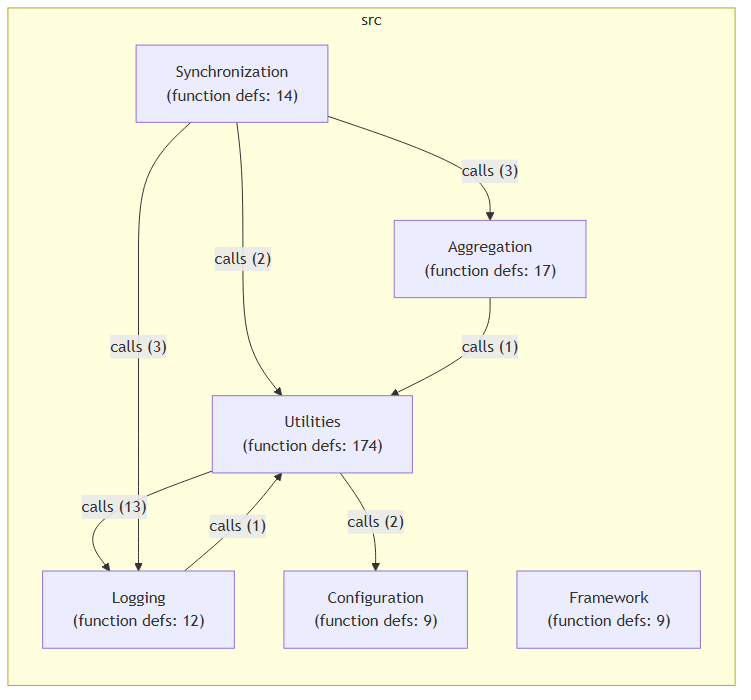
\includegraphics[width=0.85\textwidth]{figures/module-dependency.png}
  \caption{Module-level dependency structure of CPSCore (cross-directory call edges).}
  \label{fig:module-dep}
\end{figure}

\begin{figure}[htbp]
  \centering
  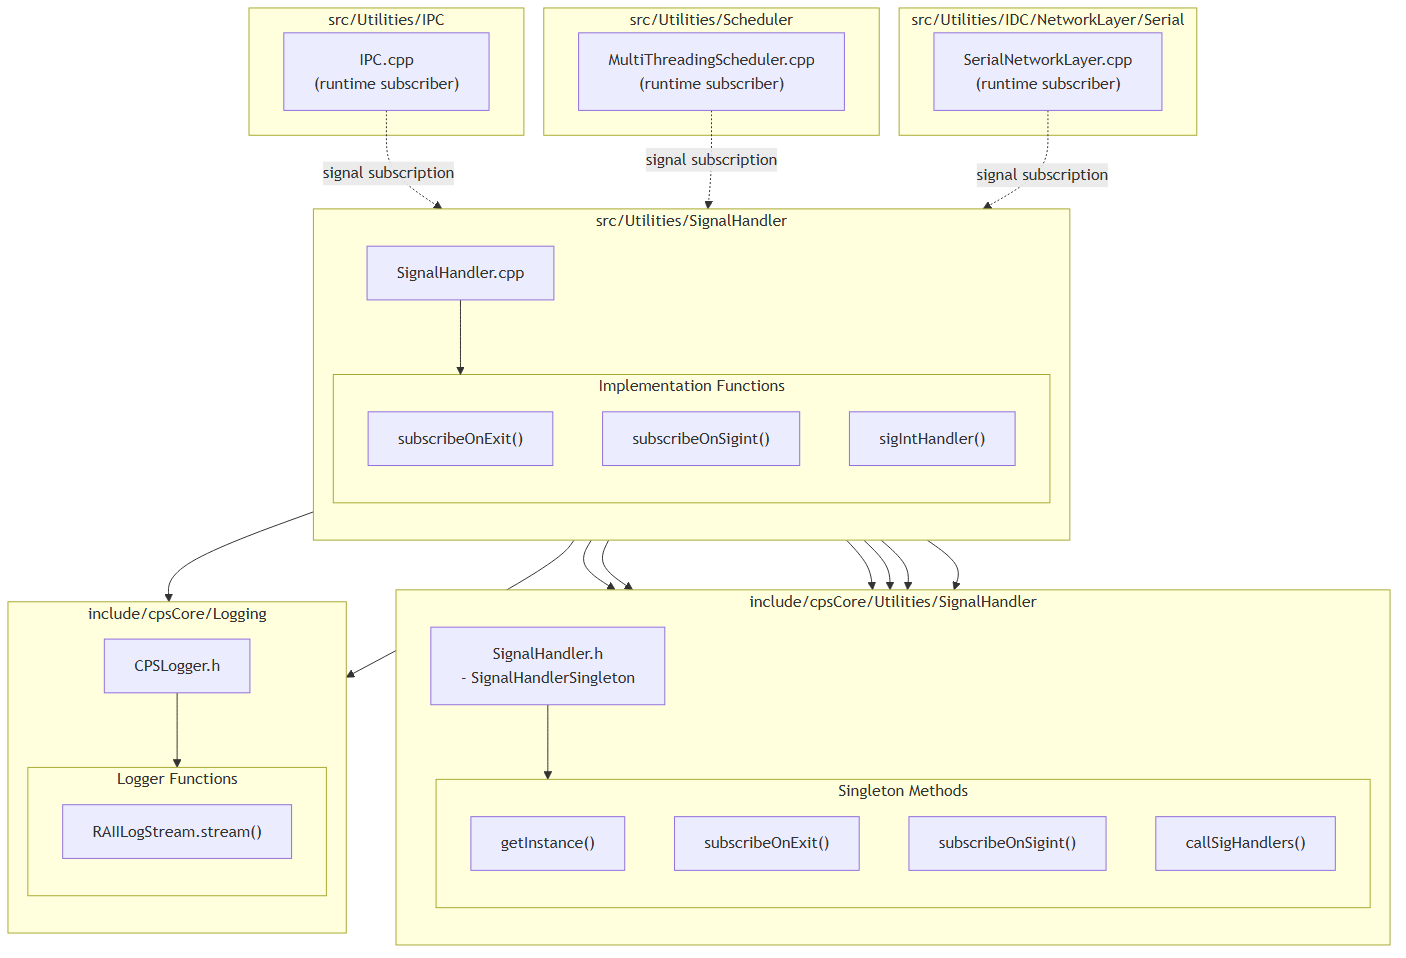
\includegraphics[width=\textwidth]{figures/signal-runtime-tracing.png}
  \caption{SignalHandler subsystem: static call edges (solid) and runtime subscriptions (dashed).}
  \label{fig:signal-tracing}
\end{figure}

\begin{figure}[htbp]
  \centering
  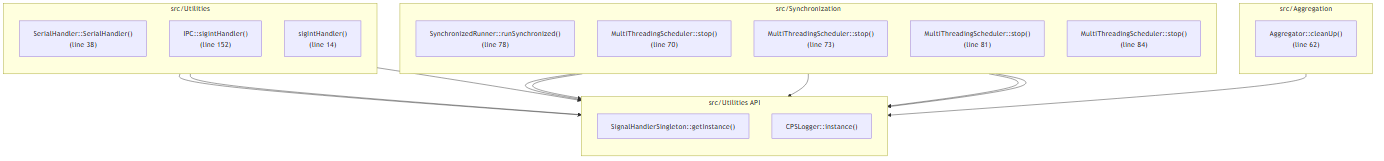
\includegraphics[width=0.9\textwidth]{figures/function-call-dependencies.png}
  \caption{Cross-module function-call dependencies to singleton APIs.}
  \label{fig:func-deps}
\end{figure}

\begin{figure}[htbp]
  \centering
  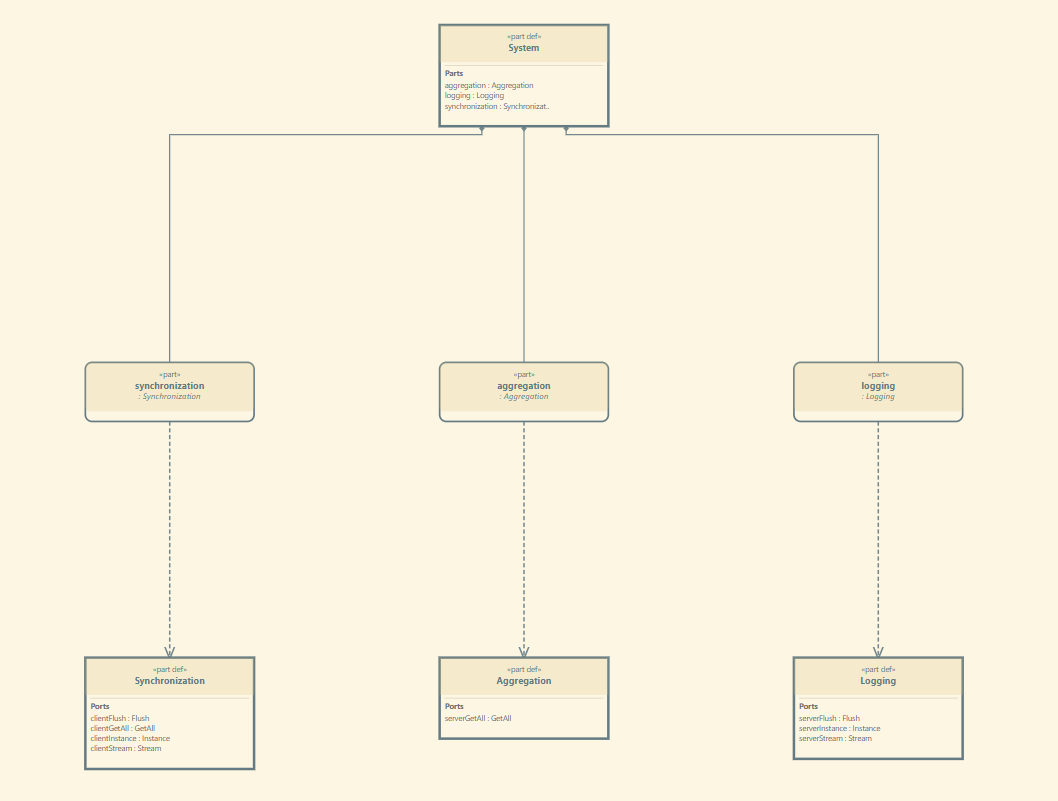
\includegraphics[width=0.75\textwidth]{figures/s1-structural.png}
  \caption{S1 structural diagram: Aggregator notification chain component connectivity.}
  \label{fig:s1-struct}
\end{figure}

\begin{figure}[htbp]
  \centering
  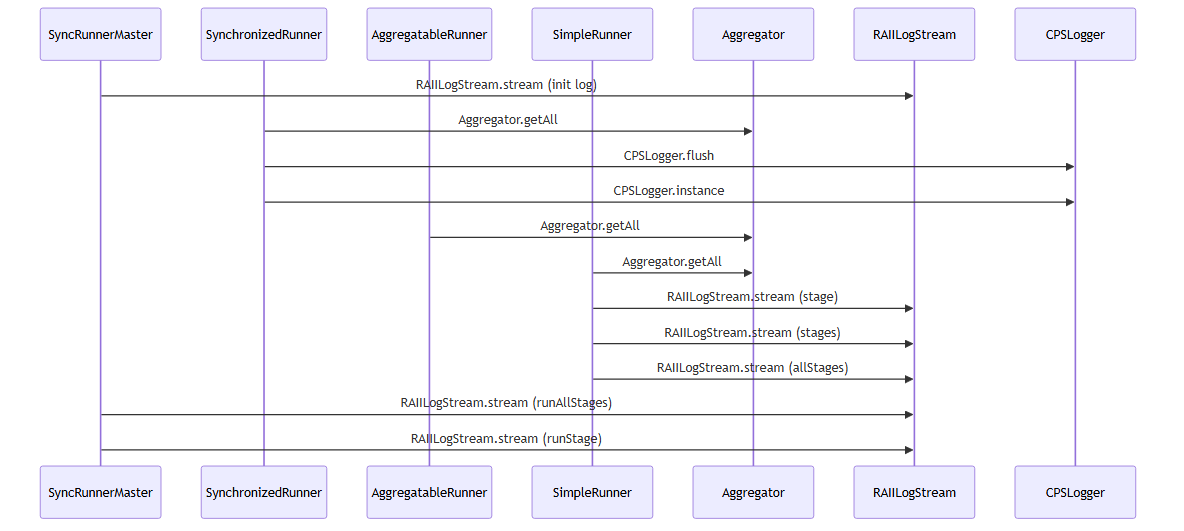
\includegraphics[width=0.85\textwidth]{figures/s1-sequence.png}
  \caption{S1 sequence diagram: Aggregator notification chain message interactions.}
  \label{fig:s1-seq}
\end{figure}

\begin{figure}[htbp]
  \centering
  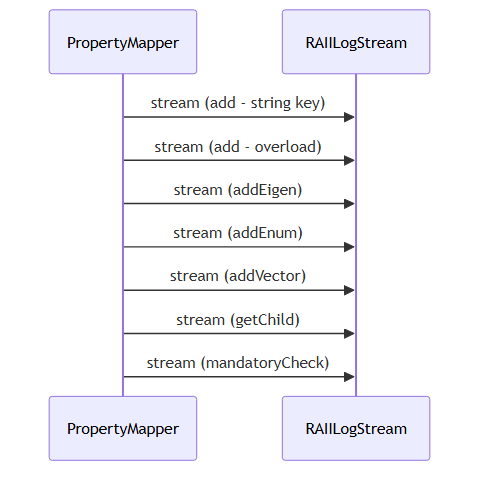
\includegraphics[width=0.6\textwidth]{figures/s2-sequence.png}
  \caption{S2 sequence diagram: Configuration property mapping (linear chain).}
  \label{fig:s2-seq}
\end{figure}

\begin{figure}[htbp]
  \centering
  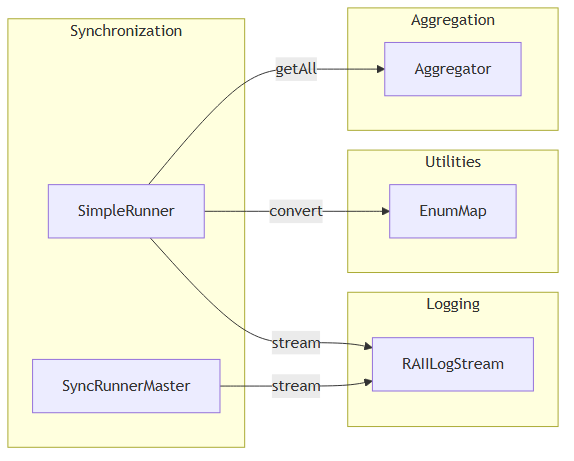
\includegraphics[width=0.75\textwidth]{figures/s3-structural.png}
  \caption{S3 structural diagram: Multi-component runner fan-out connectivity.}
  \label{fig:s3-struct}
\end{figure}

\begin{figure}[htbp]
  \centering
  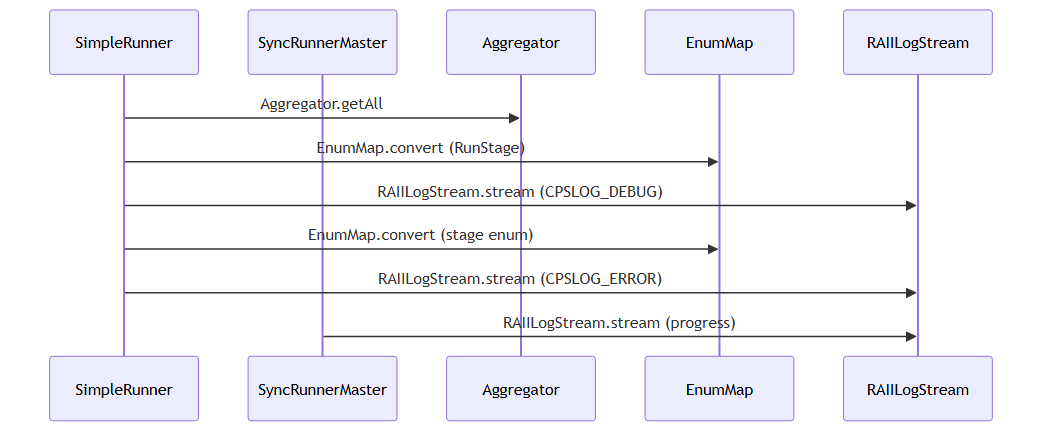
\includegraphics[width=0.85\textwidth]{figures/s3-sequence.png}
  \caption{S3 sequence diagram: Multi-component runner orchestration.}
  \label{fig:s3-seq}
\end{figure}

\section{H2 Qualitative Arm: Per-Rater Decomposition}
\label{sec:appendix-h2-perrater}

This appendix records the full per-rater decomposition and free-text
analysis of the blinded expert rating study summarised in
\cref{sec:h2-qual}. The aggregate results (\cref{tab:h2-qual-results}) and
the headline finding are given in the main text; the detail below supports
the claim that the accuracy/readability effect is unanimous in direction
and that the only genuine split is usefulness on~S2.

Expanding the panel from two to six raters did not change the direction of
the effect, but it did surface real heterogeneity that a two-rater sample
could not. One rater (R4) consistently rated the two conditions closer
together than the other five, accounted for two of the six accuracy ties
(S2, S3) and one of the six usefulness ties (S1), and produced the
dataset's only reversal: rating full instrumentation's usefulness
\emph{above} guided's on S2 ($4$ vs.\ $3$). The remaining three ties (S2
usefulness, from raters R1--R3) are a separate, converging signal,
discussed below. No rater ever rated full instrumentation higher on
accuracy or readability, on any scenario: that effect is unanimous in
direction across all six raters (never reversed, though twice tied), while
the usefulness effect is unanimous on S1 and S3 and genuinely mixed on S2.

The free-text comments explain why.
For S1 and S3, five of the six raters independently described the guided
diagram as retaining only the components named in the scenario context and
starting at the correct point in the sequence, while the
full-instrumentation diagram was called more complete but cluttered with
additional \texttt{stream} events that are just streaming and not
obviously relevant without prior codebase knowledge. One rater (R1), while
still preferring the guided diagram overall, flagged a residual critique
of it directly: an \texttt{instance} call retained in the guided S1
diagram was, in their words, ``also superfluous.'' This is a useful
reminder that H2's noise$=0$ result (\cref{sec:h2-results}) is scoped to
the reference set used for scoring, not to what a domain expert reading
the diagram cold considers extraneous. The two need not coincide, and
here, for at least one rater, they did not.

S2 shows the same underlying pattern with the surface direction reversed:
the guided diagram collapses seven repeated
\texttt{Configuration}$\to$\texttt{Logging} property-read calls into a
single edge (\cref{tab:h2-per-scenario}), and five of the six raters rated
this collapsed diagram as more accurate and more readable because it
matches the two components named in the scenario context. Usefulness is
where the panel genuinely splits. Three raters (R1--R3) rated usefulness
an exact tie, each independently giving the same reason in their
free-text comments: collapsing the repeated reads into one edge loses the
\emph{count} of property reads, information they considered relevant to
debugging even though it played no part in their accuracy or readability
judgement. A fourth rater (R4) went further and rated full instrumentation
\emph{more} useful on S2, commenting that with the guided diagram alone
``it is not clear what triggers a logging event.'' This is a distinct usability
concern (about explaining a trigger condition) rather than a repeat of the
counting concern raised by R1--R3. Only two raters (R5, R6) rated guided as
more useful outright on S2. Usefulness on S2 is therefore best read as a
genuine three-way split (tied, reversed, and in-favour-of-guided) rather
than a clean preference in either direction: a more precise, and more
defensible, characterisation than the exact 2-rater tie originally
reported from the smaller panel.

Several raters also converged independently on the same practical
suggestions for handling high-volume \texttt{stream} events. Two raters
(R3, R6) suggested a way to toggle, filter, or visually distinguish them
rather than always including or always omitting them, and a third (R2)
suggested recording the specific property value emitted by each
\texttt{stream} call, so that the collapsed S2 edge would be as useful for
debugging as the uncollapsed one without losing its readability advantage.
R3 additionally proposed a two-stage workflow: use the
full-instrumentation diagram to see where an interaction sits within the
broader flow, then use the guided diagram to reason about the scenario
itself. This reframes full instrumentation not as a failed alternative to
guided instrumentation, but as a complementary, coarser-grained view.

\section{SysML v2 Generated Diagrams}
\label{sec:appendix-sysmlv2}

The following figures show the SysML v2 diagrams generated by the pipeline
for the CPSCore case study. These include both structural (component
connectivity) diagrams and sequence (interaction flow) diagrams produced
under condition C5 (full pipeline).

\subsection{Structural Diagrams}

\begin{figure}[htbp]
  \centering
  
\includegraphics[width=\textwidth]{figures/sysmlv2 diagrams/structure.png}
  \caption{SysML v2 structural diagram: complete CPSCore component model showing
    all part definitions and their interface connections.}
  \label{fig:sysml-structure}
\end{figure}

\begin{figure}[htbp]
  \centering
  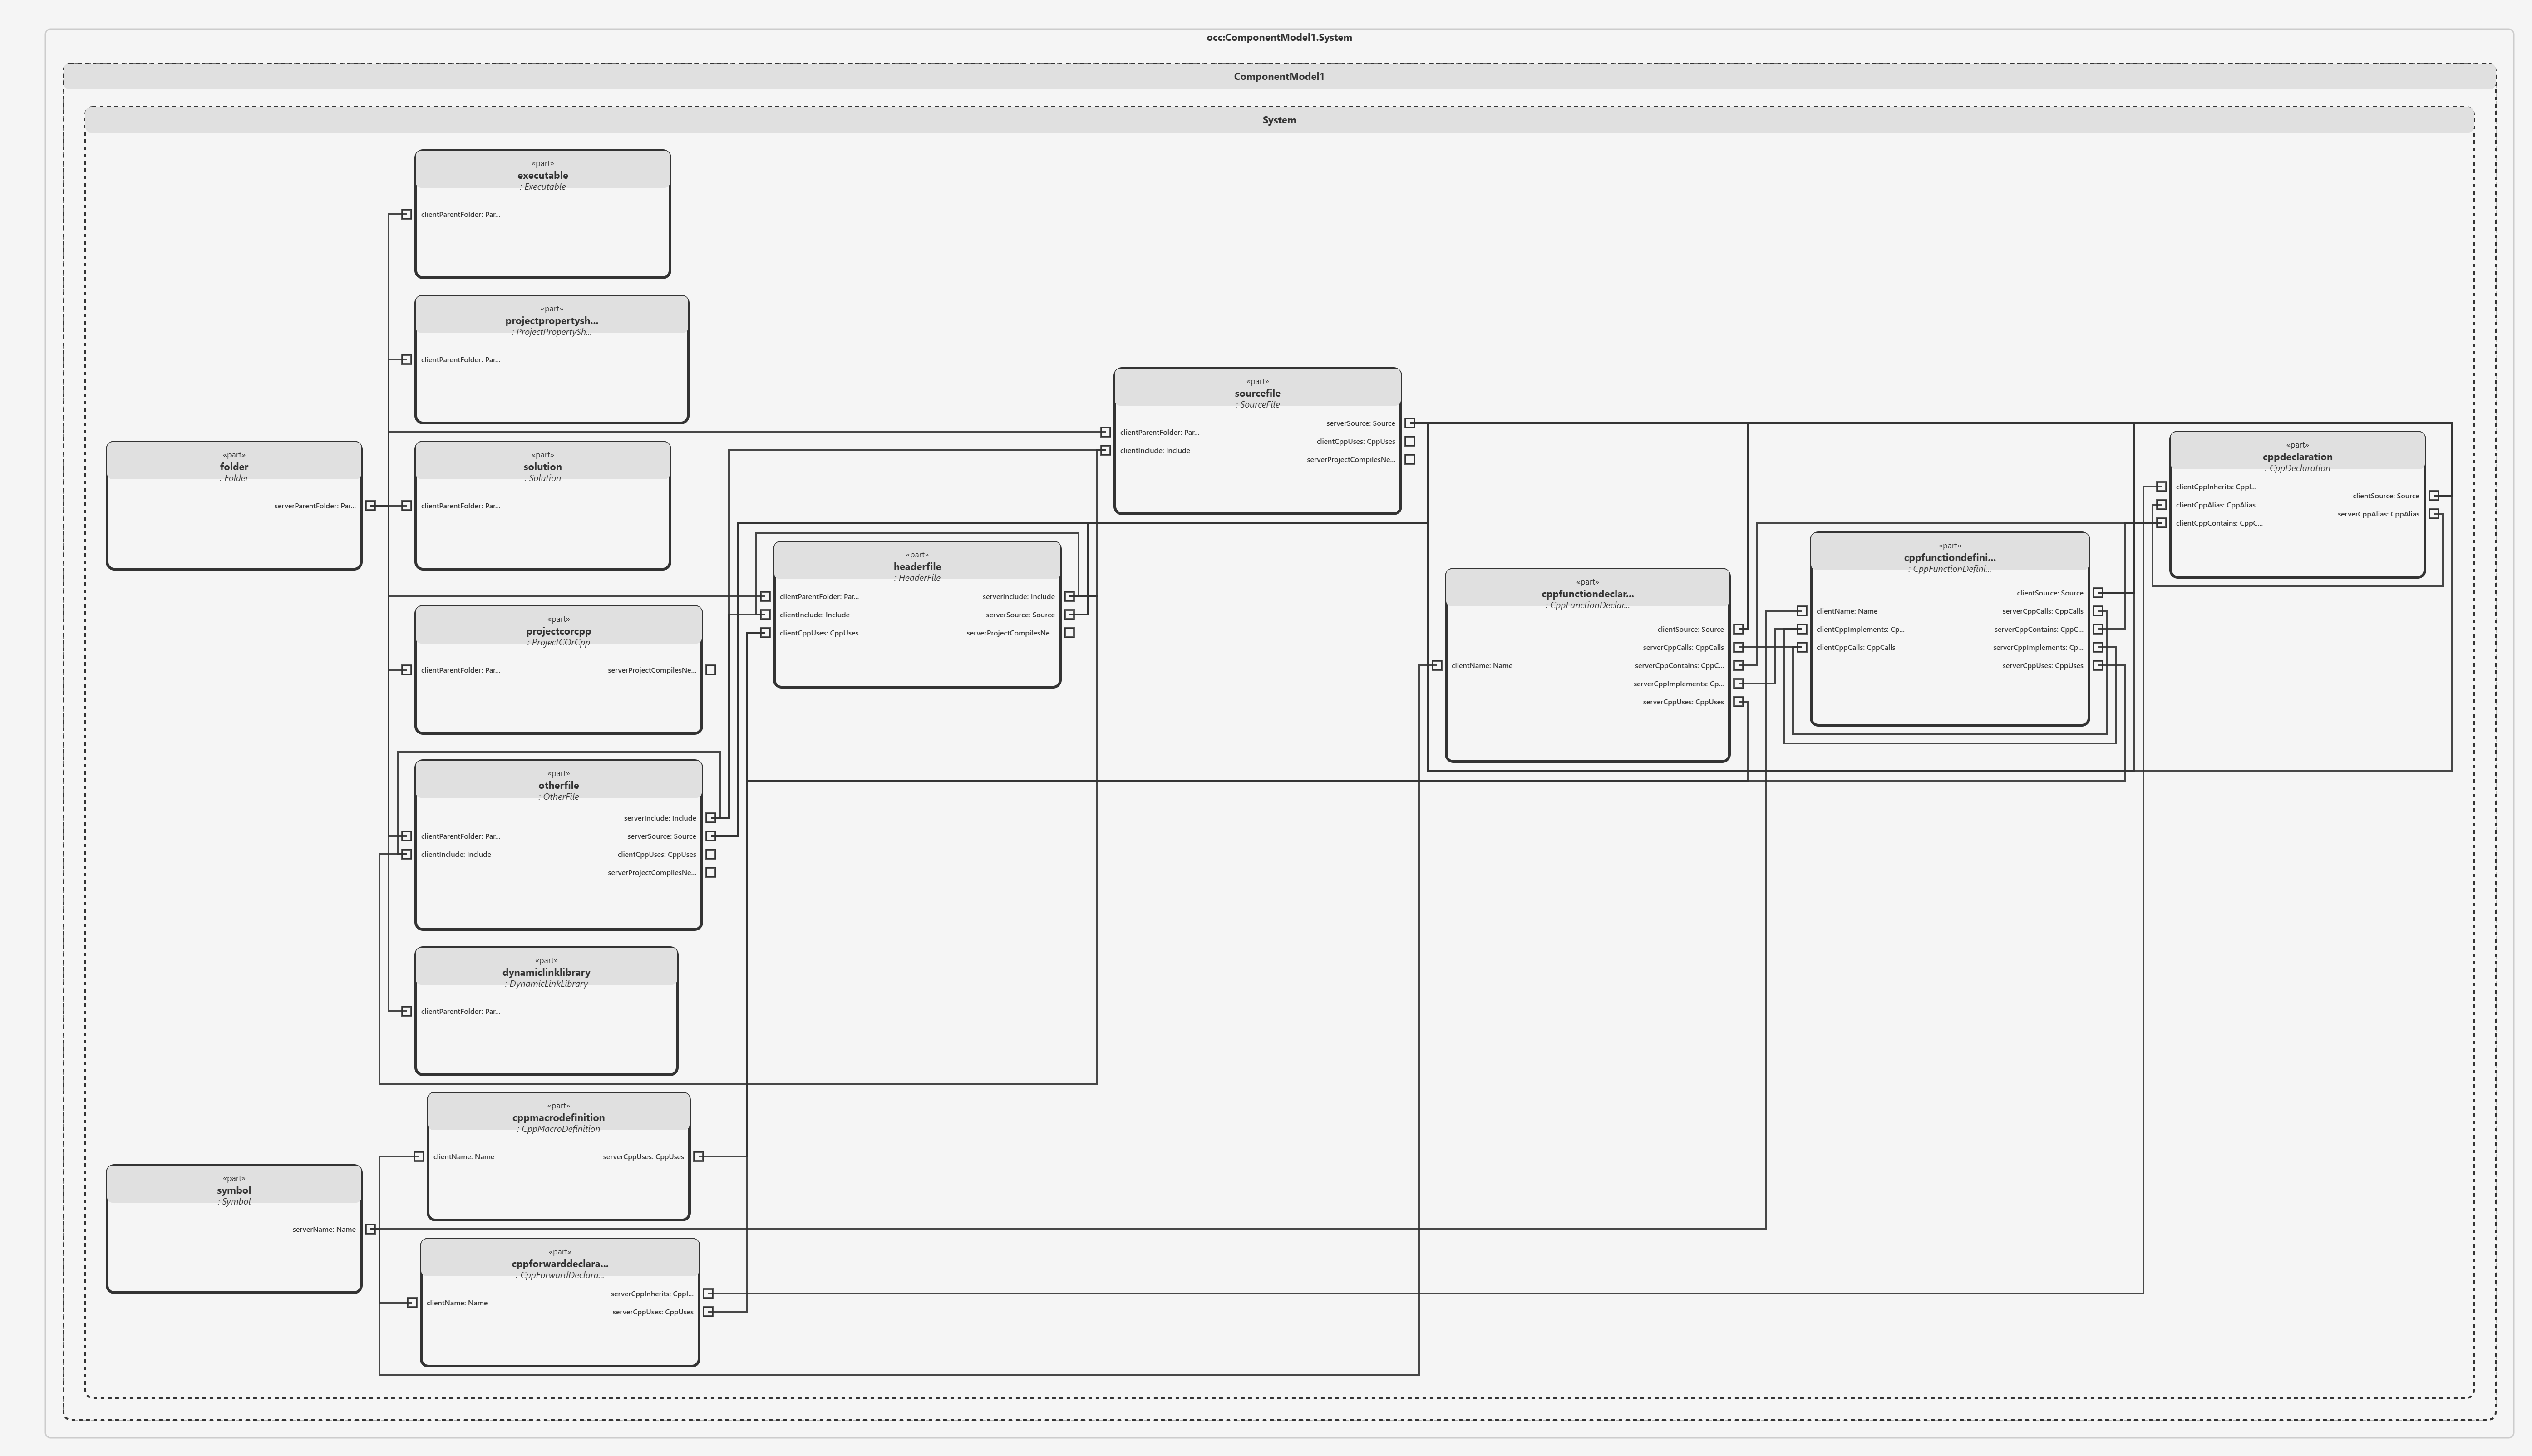
\includegraphics[width=\textwidth]{figures/sysmlv2 diagrams/connections.png}
  \caption{SysML v2 connections diagram: node-type hierarchy and property graph
    schema relationships between all 13 node labels.}
  \label{fig:sysml-connections}
\end{figure}

\subsection{Sequence Diagrams}

\begin{figure}[htbp]
  \centering
  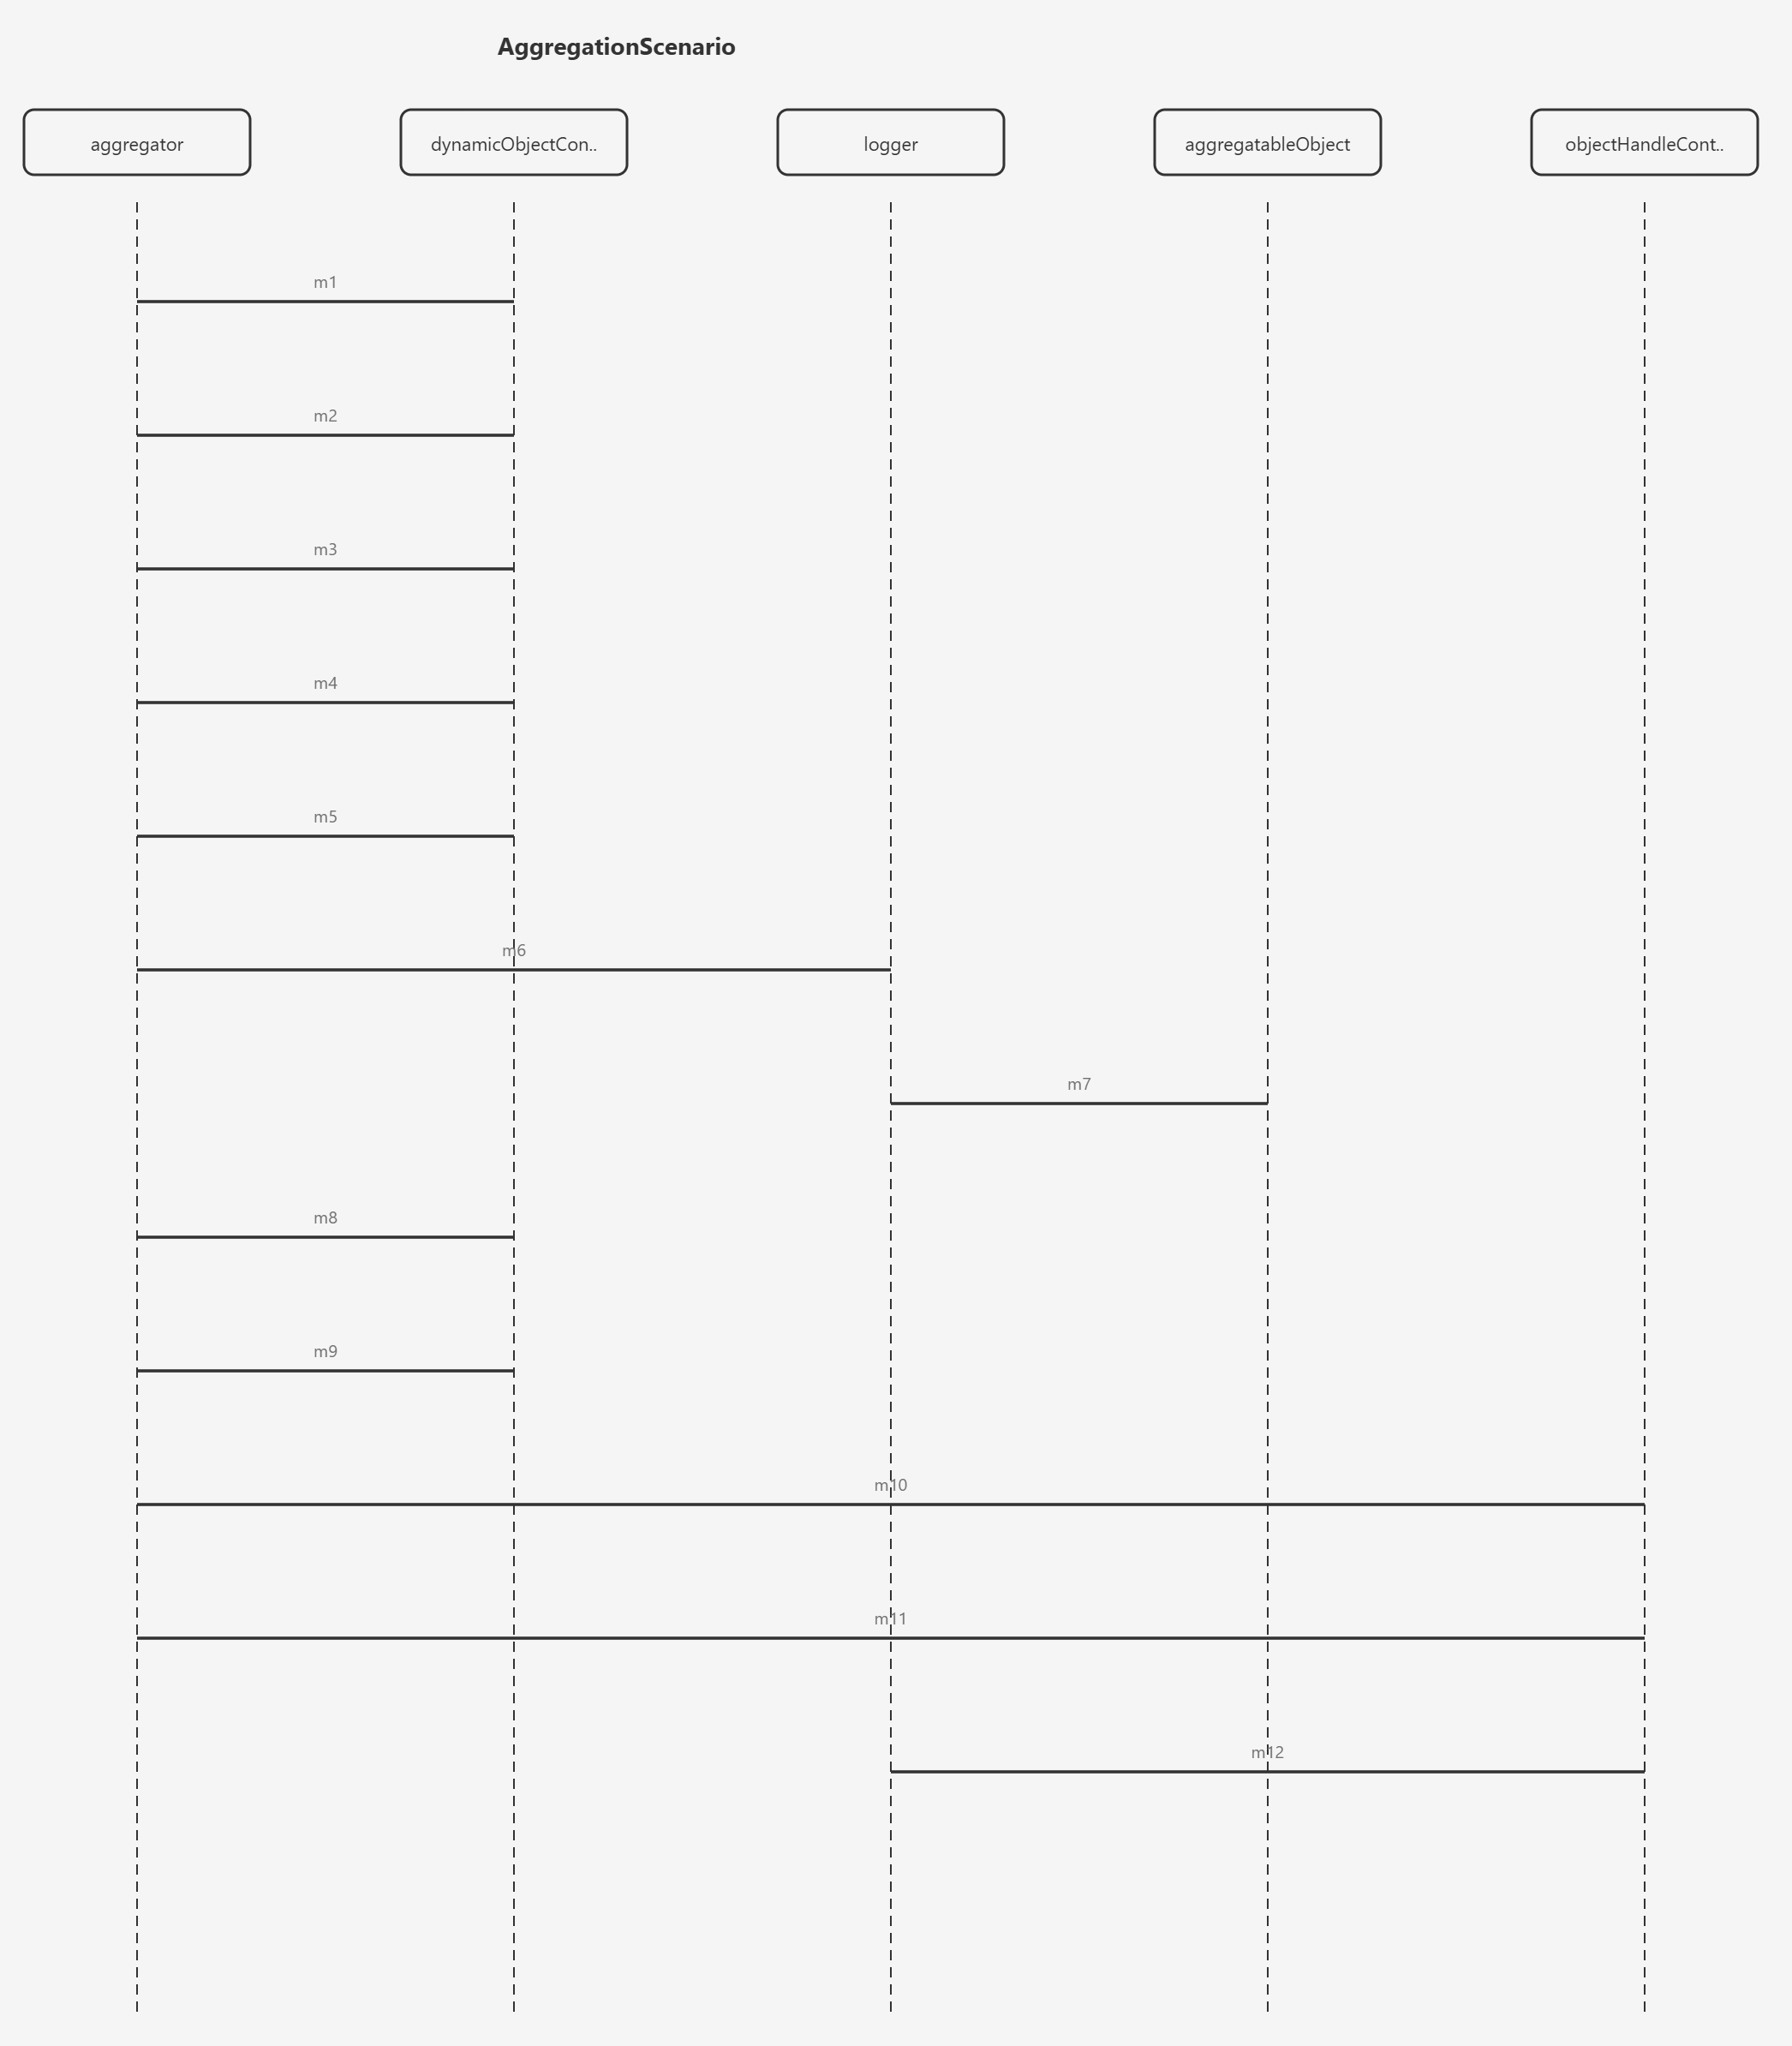
\includegraphics[width=0.9\textwidth]{figures/sysmlv2 diagrams/aggregationFlow.png}
  \caption{SysML v2 sequence diagram: Aggregation scenario showing component
    wiring and lifecycle interactions (Aggregator, DynamicObjectContainer,
    Logger, AggregatableObject).}
  \label{fig:sysml-aggregation}
\end{figure}

\begin{figure}[htbp]
  \centering
  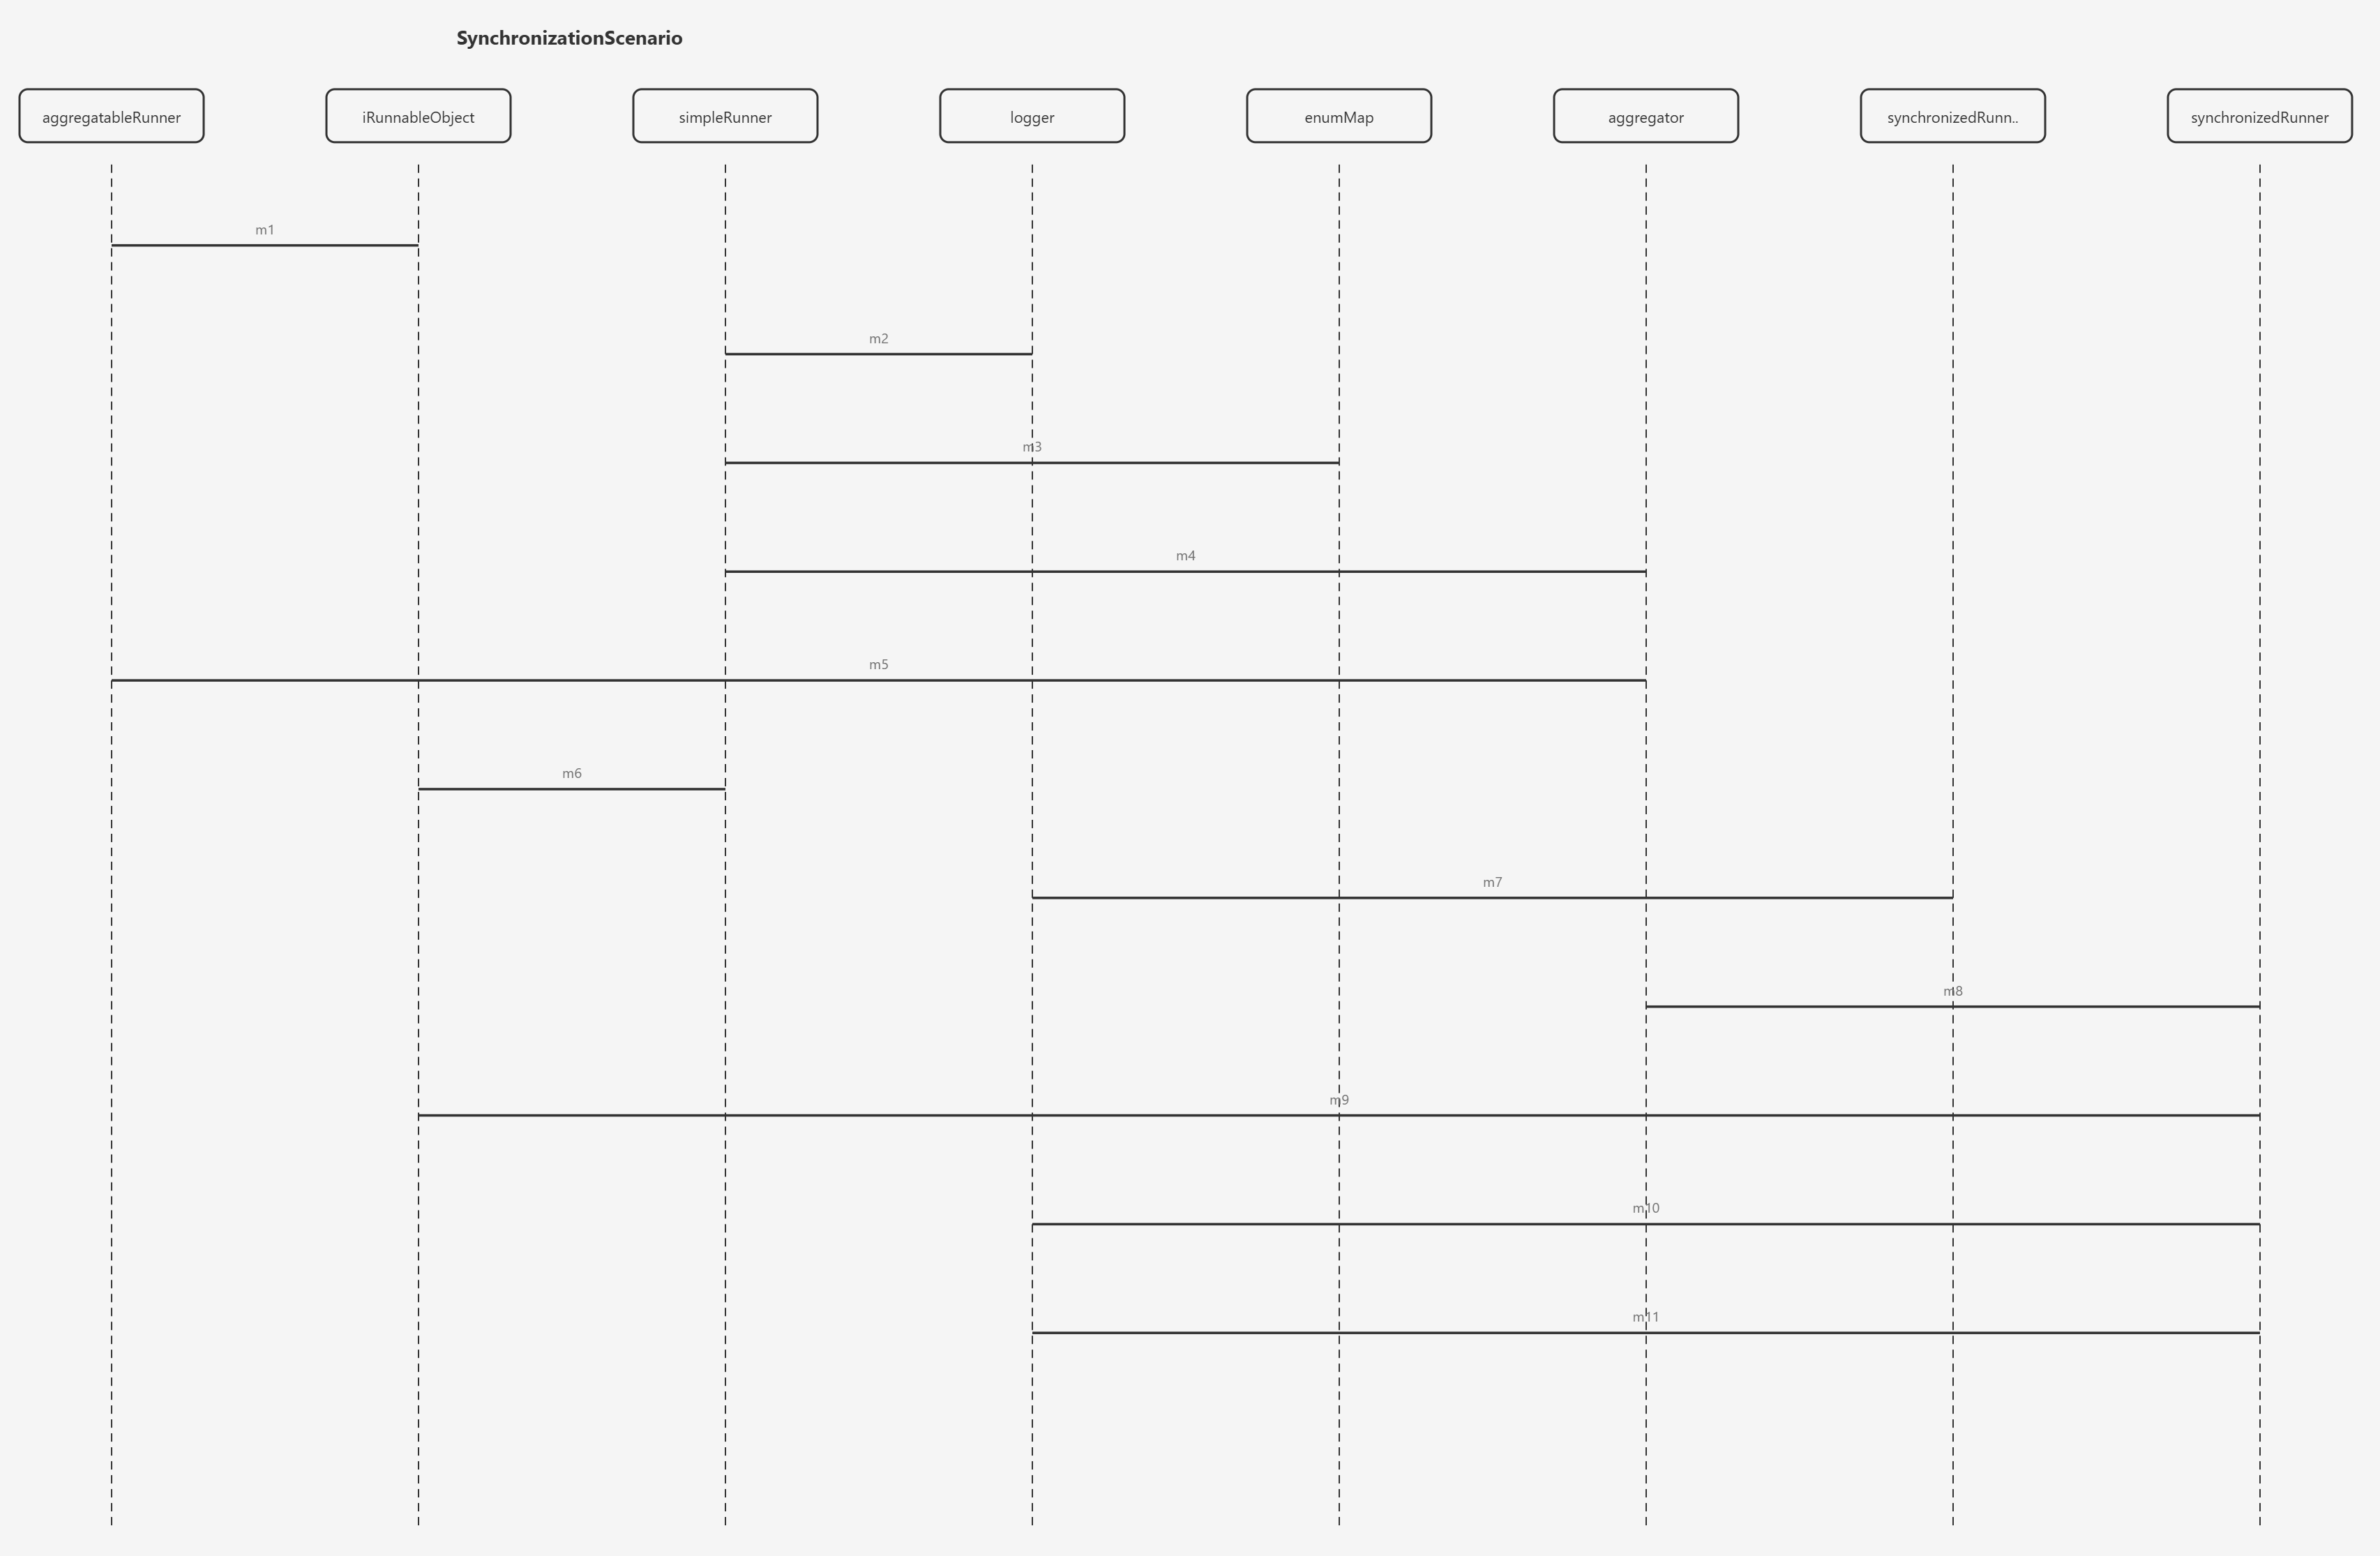
\includegraphics[width=0.9\textwidth]{figures/sysmlv2 diagrams/synchronizationFlow.png}
  \caption{SysML v2 sequence diagram: Synchronization scenario showing
    run-stage scheduling interactions between AggregatableRunner,
    IRunnableObject, SimpleRunner, Logger, EnumMap, Aggregator,
    SynchronizedRunnerMaster, and SynchronizedRunner.}
  \label{fig:sysml-synchronization}
\end{figure}

\begin{figure}[H]
  \centering
  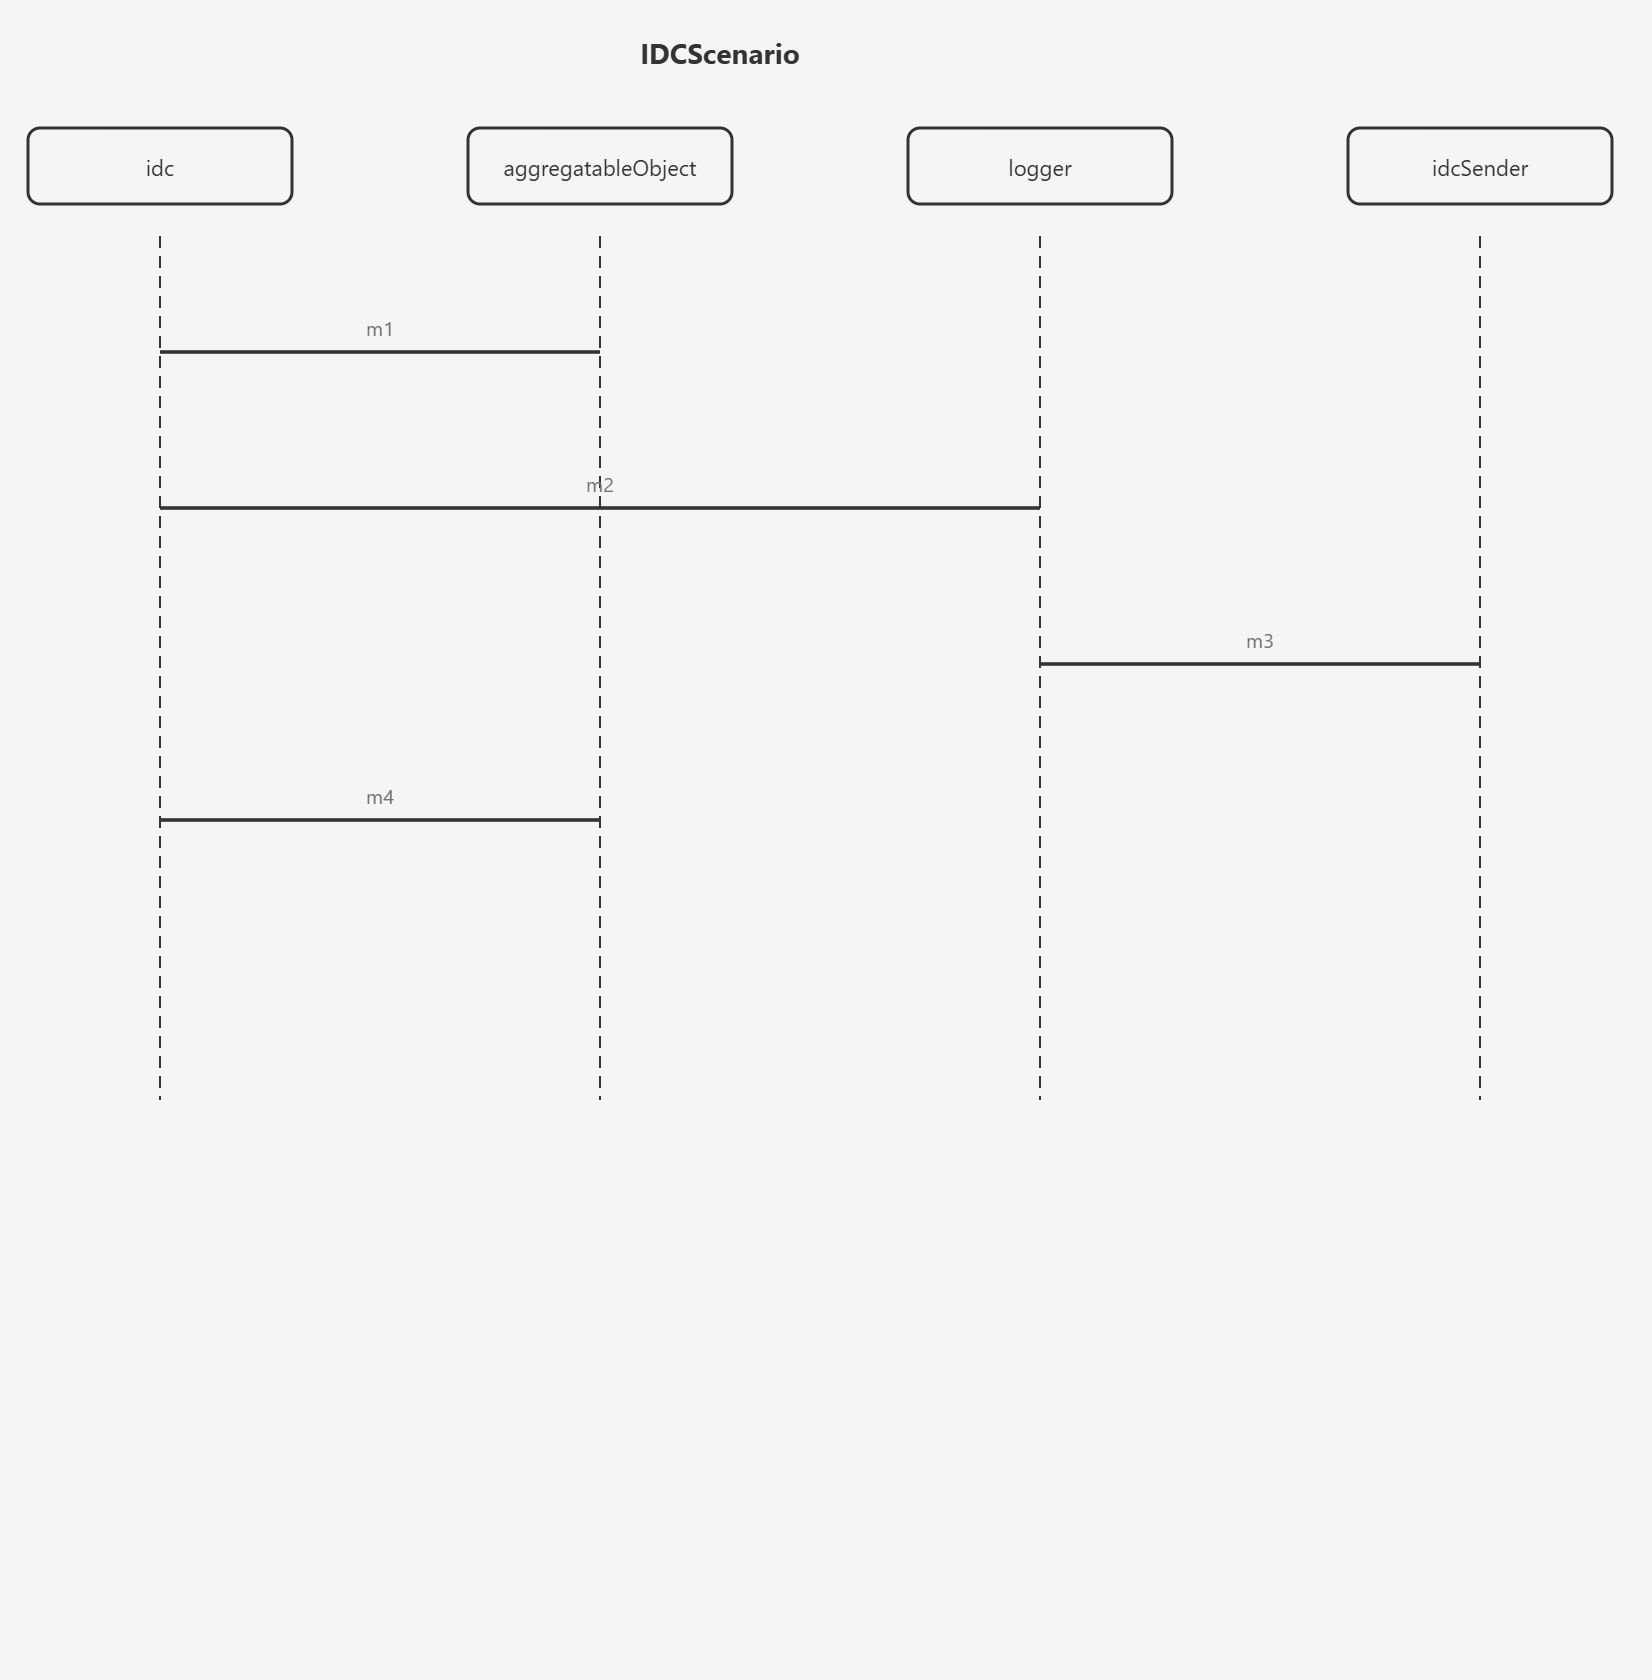
\includegraphics[width=0.85\textwidth]{figures/sysmlv2 diagrams/idcFlow.png}
  \caption{SysML v2 sequence diagram: IDC scenario showing inter-component
    communication through the IDC abstraction layer (IDC, AggregatableObject,
    Logger, IDCSender).}
  \label{fig:sysml-idc}
\end{figure}

\begin{figure}[htbp]
  \centering
  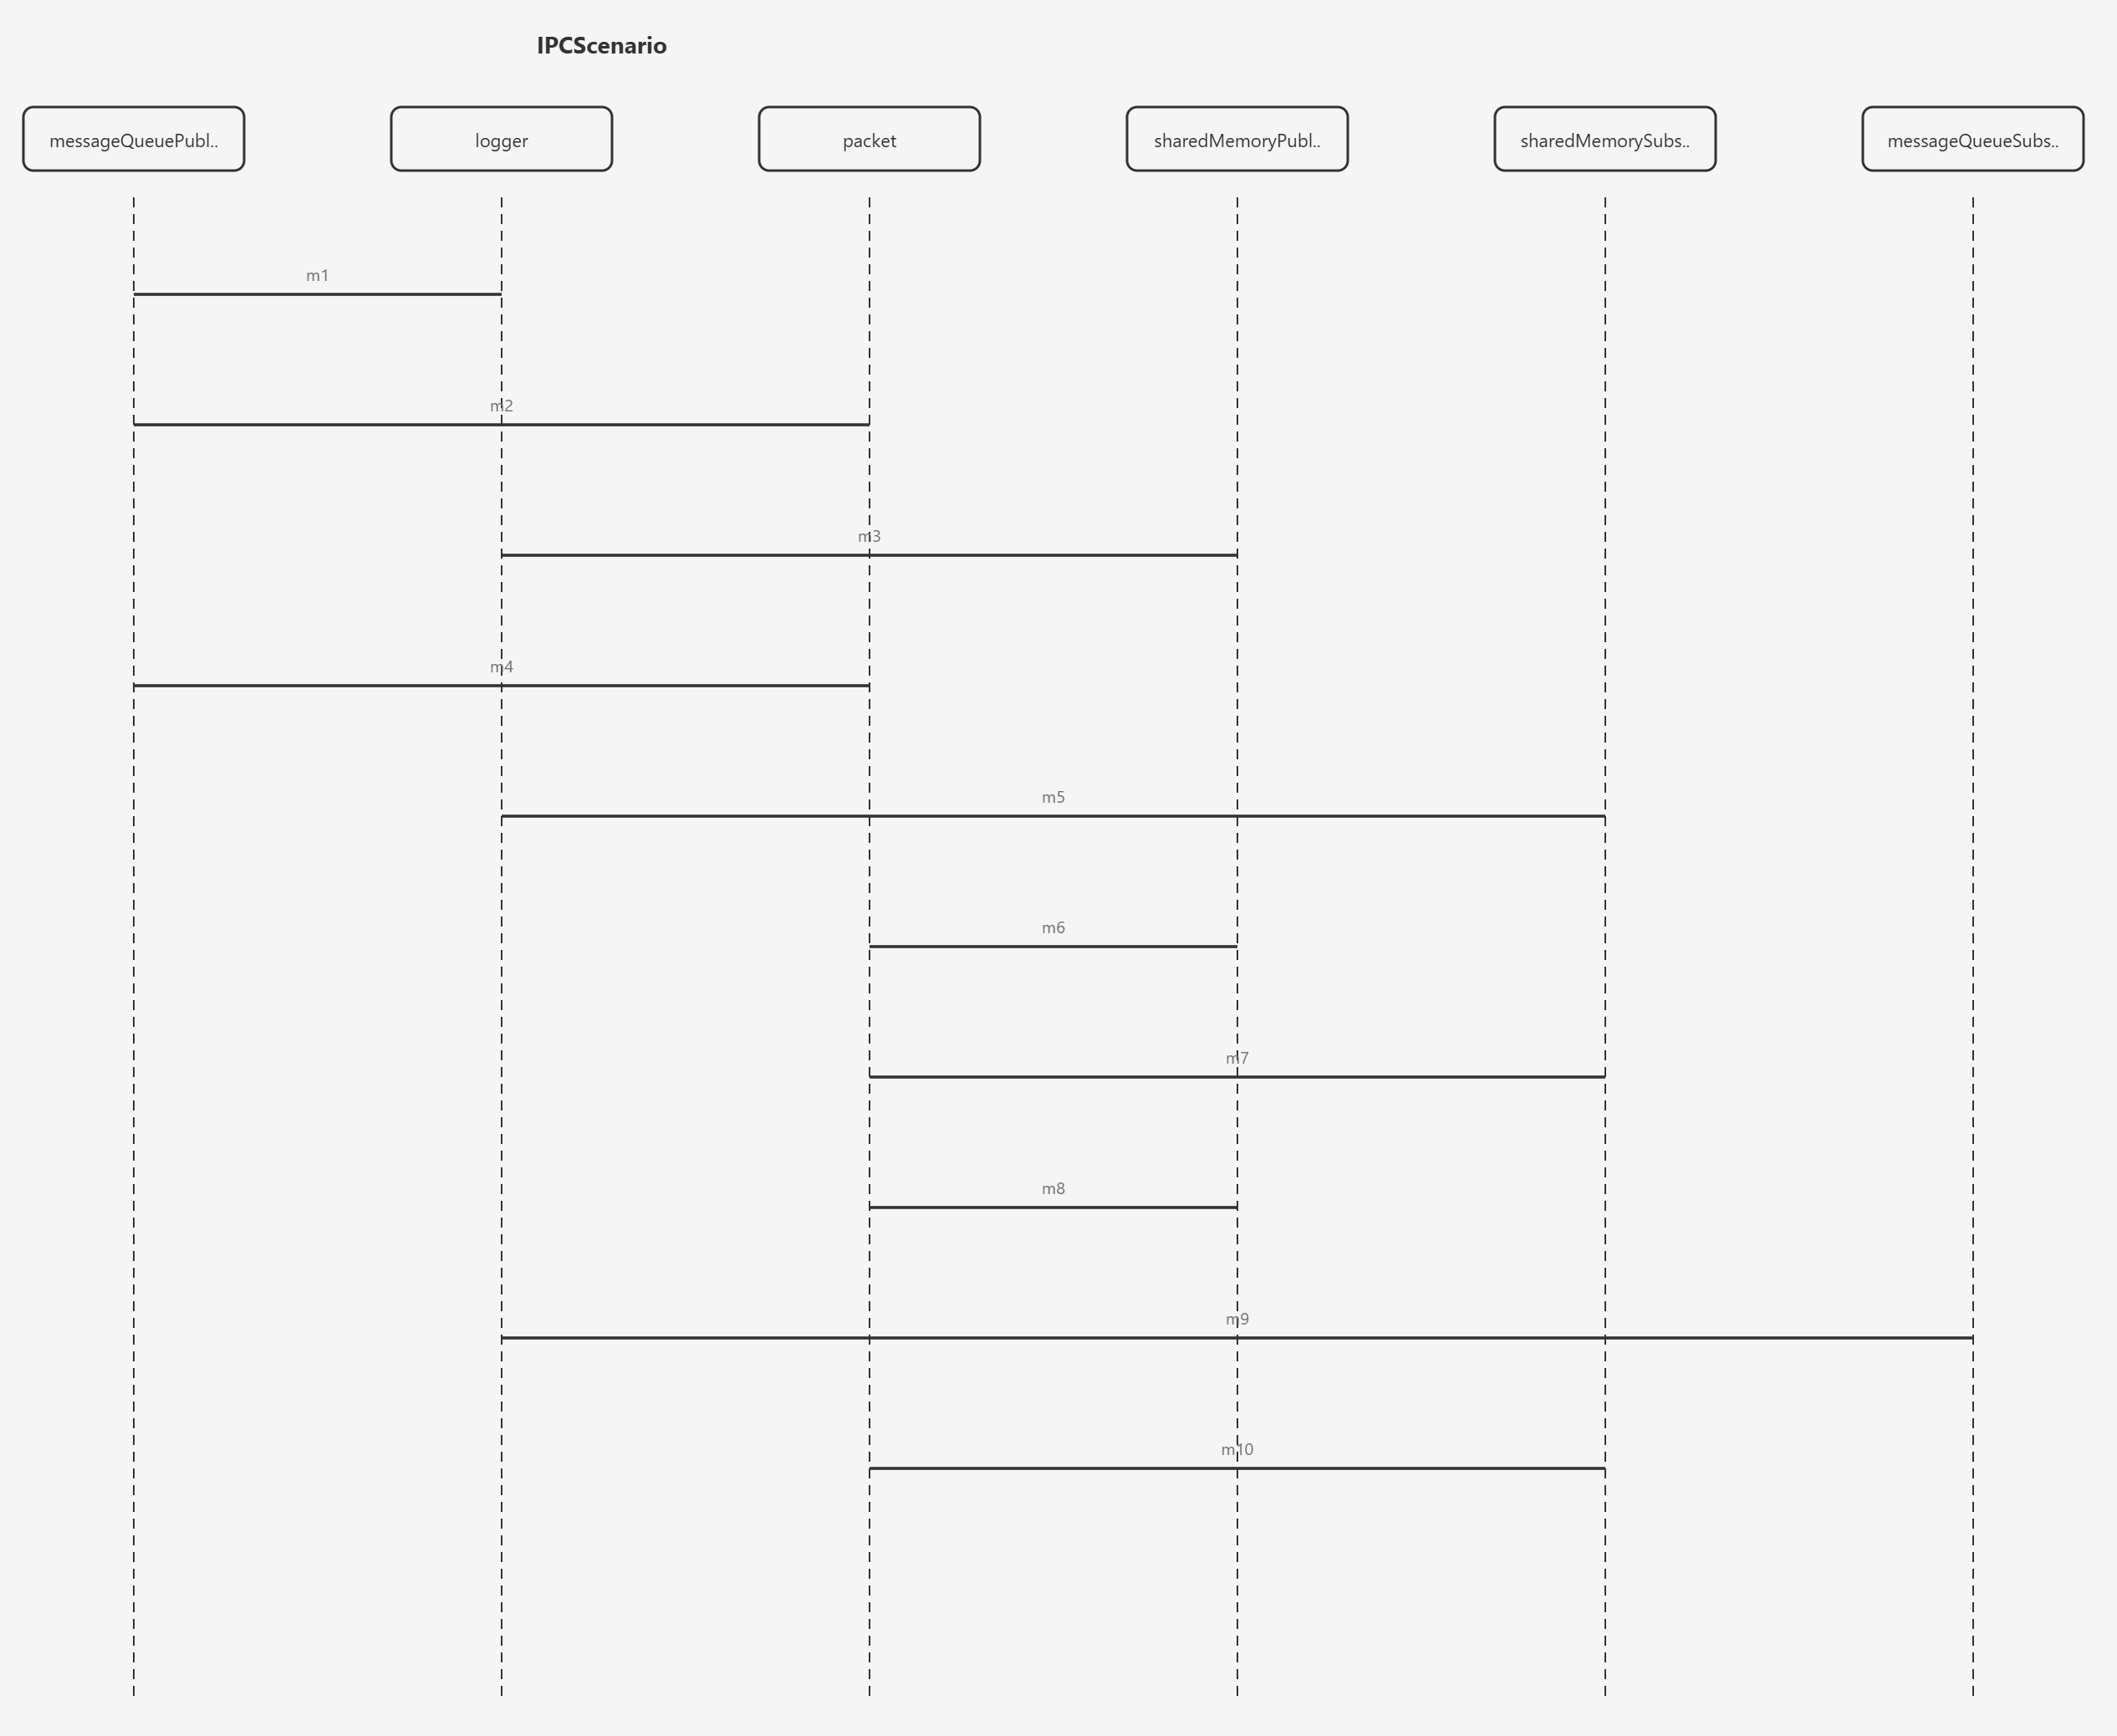
\includegraphics[width=0.9\textwidth]{figures/sysmlv2 diagrams/ipcFlow.png}
  \caption{SysML v2 sequence diagram: IPC scenario showing message queue and
    shared memory publisher/subscriber interactions (MessageQueuePublisher,
    Logger, Packet, SharedMemoryPublisher, SharedMemorySubscriber,
    MessageQueueSubscriber).}
  \label{fig:sysml-ipc}
\end{figure}

\begin{figure}[htbp]
  \centering
  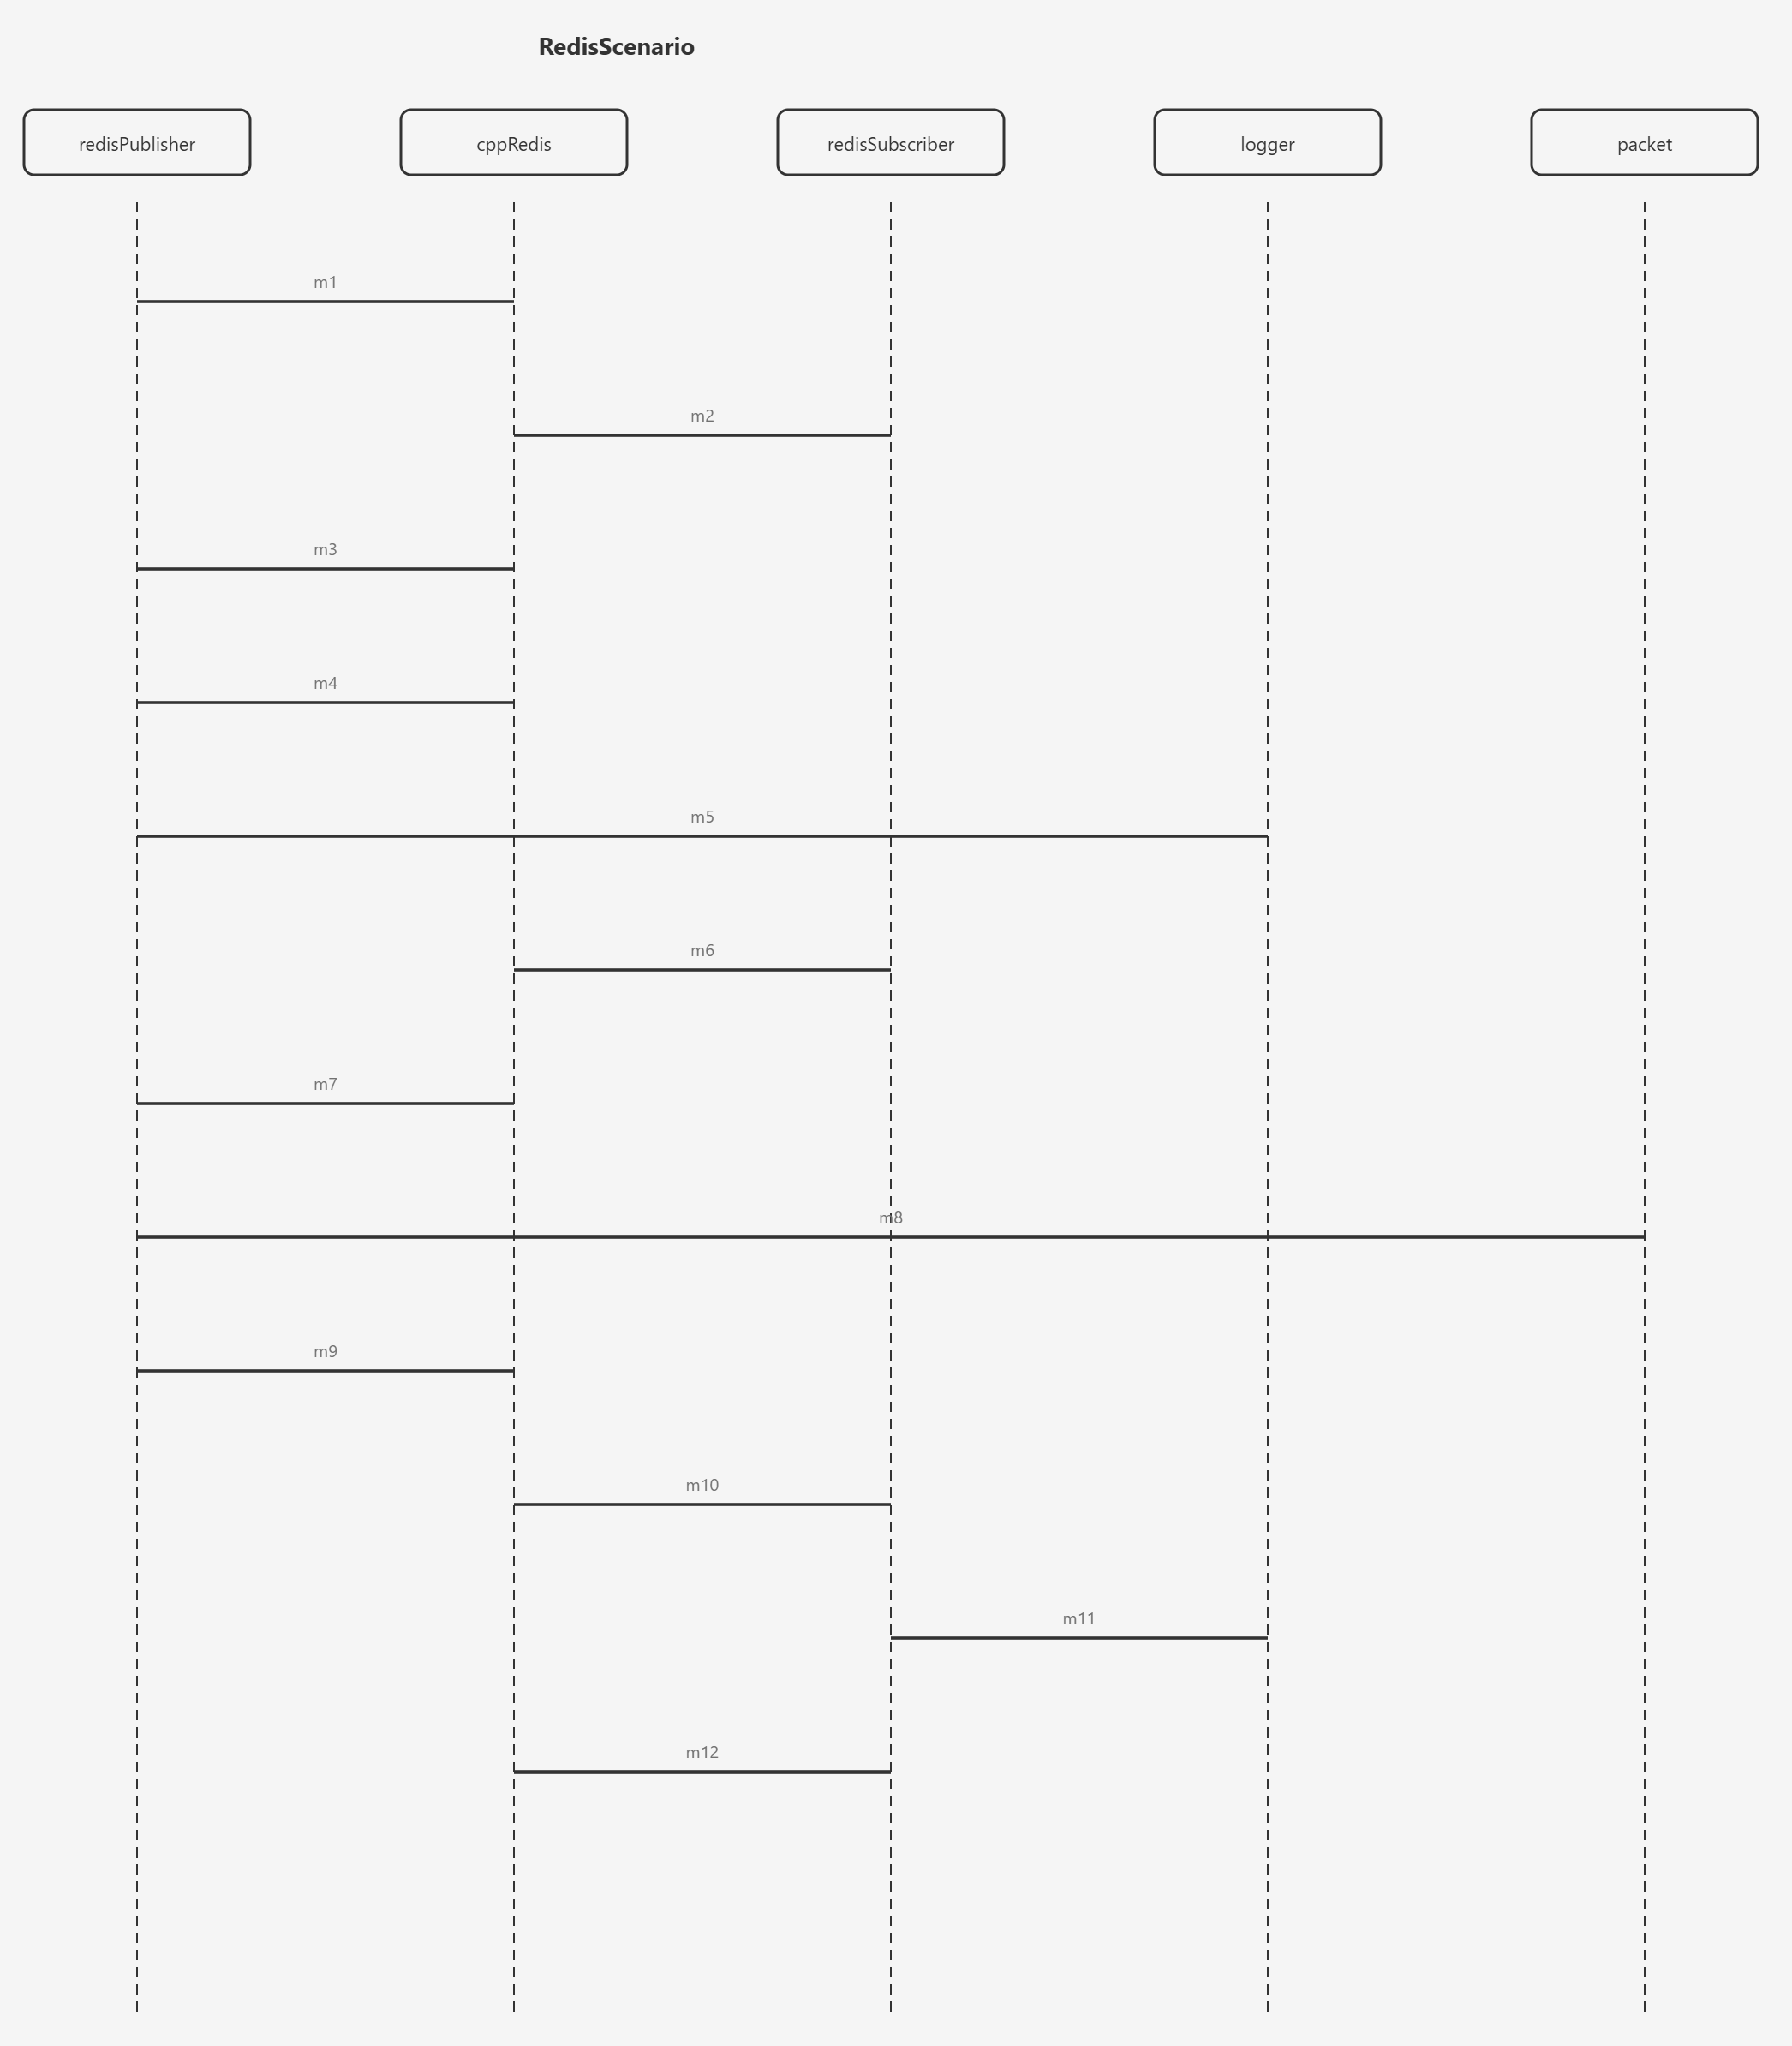
\includegraphics[width=0.9\textwidth]{figures/sysmlv2 diagrams/redisFlow.png}
  \caption{SysML v2 sequence diagram: Redis scenario showing the Redis-based
    publish-subscribe communication path (RedisPublisher, CppRedis,
    RedisSubscriber, Logger, Packet).}
  \label{fig:sysml-redis}
\end{figure}

\begin{figure}[H]
  \centering
  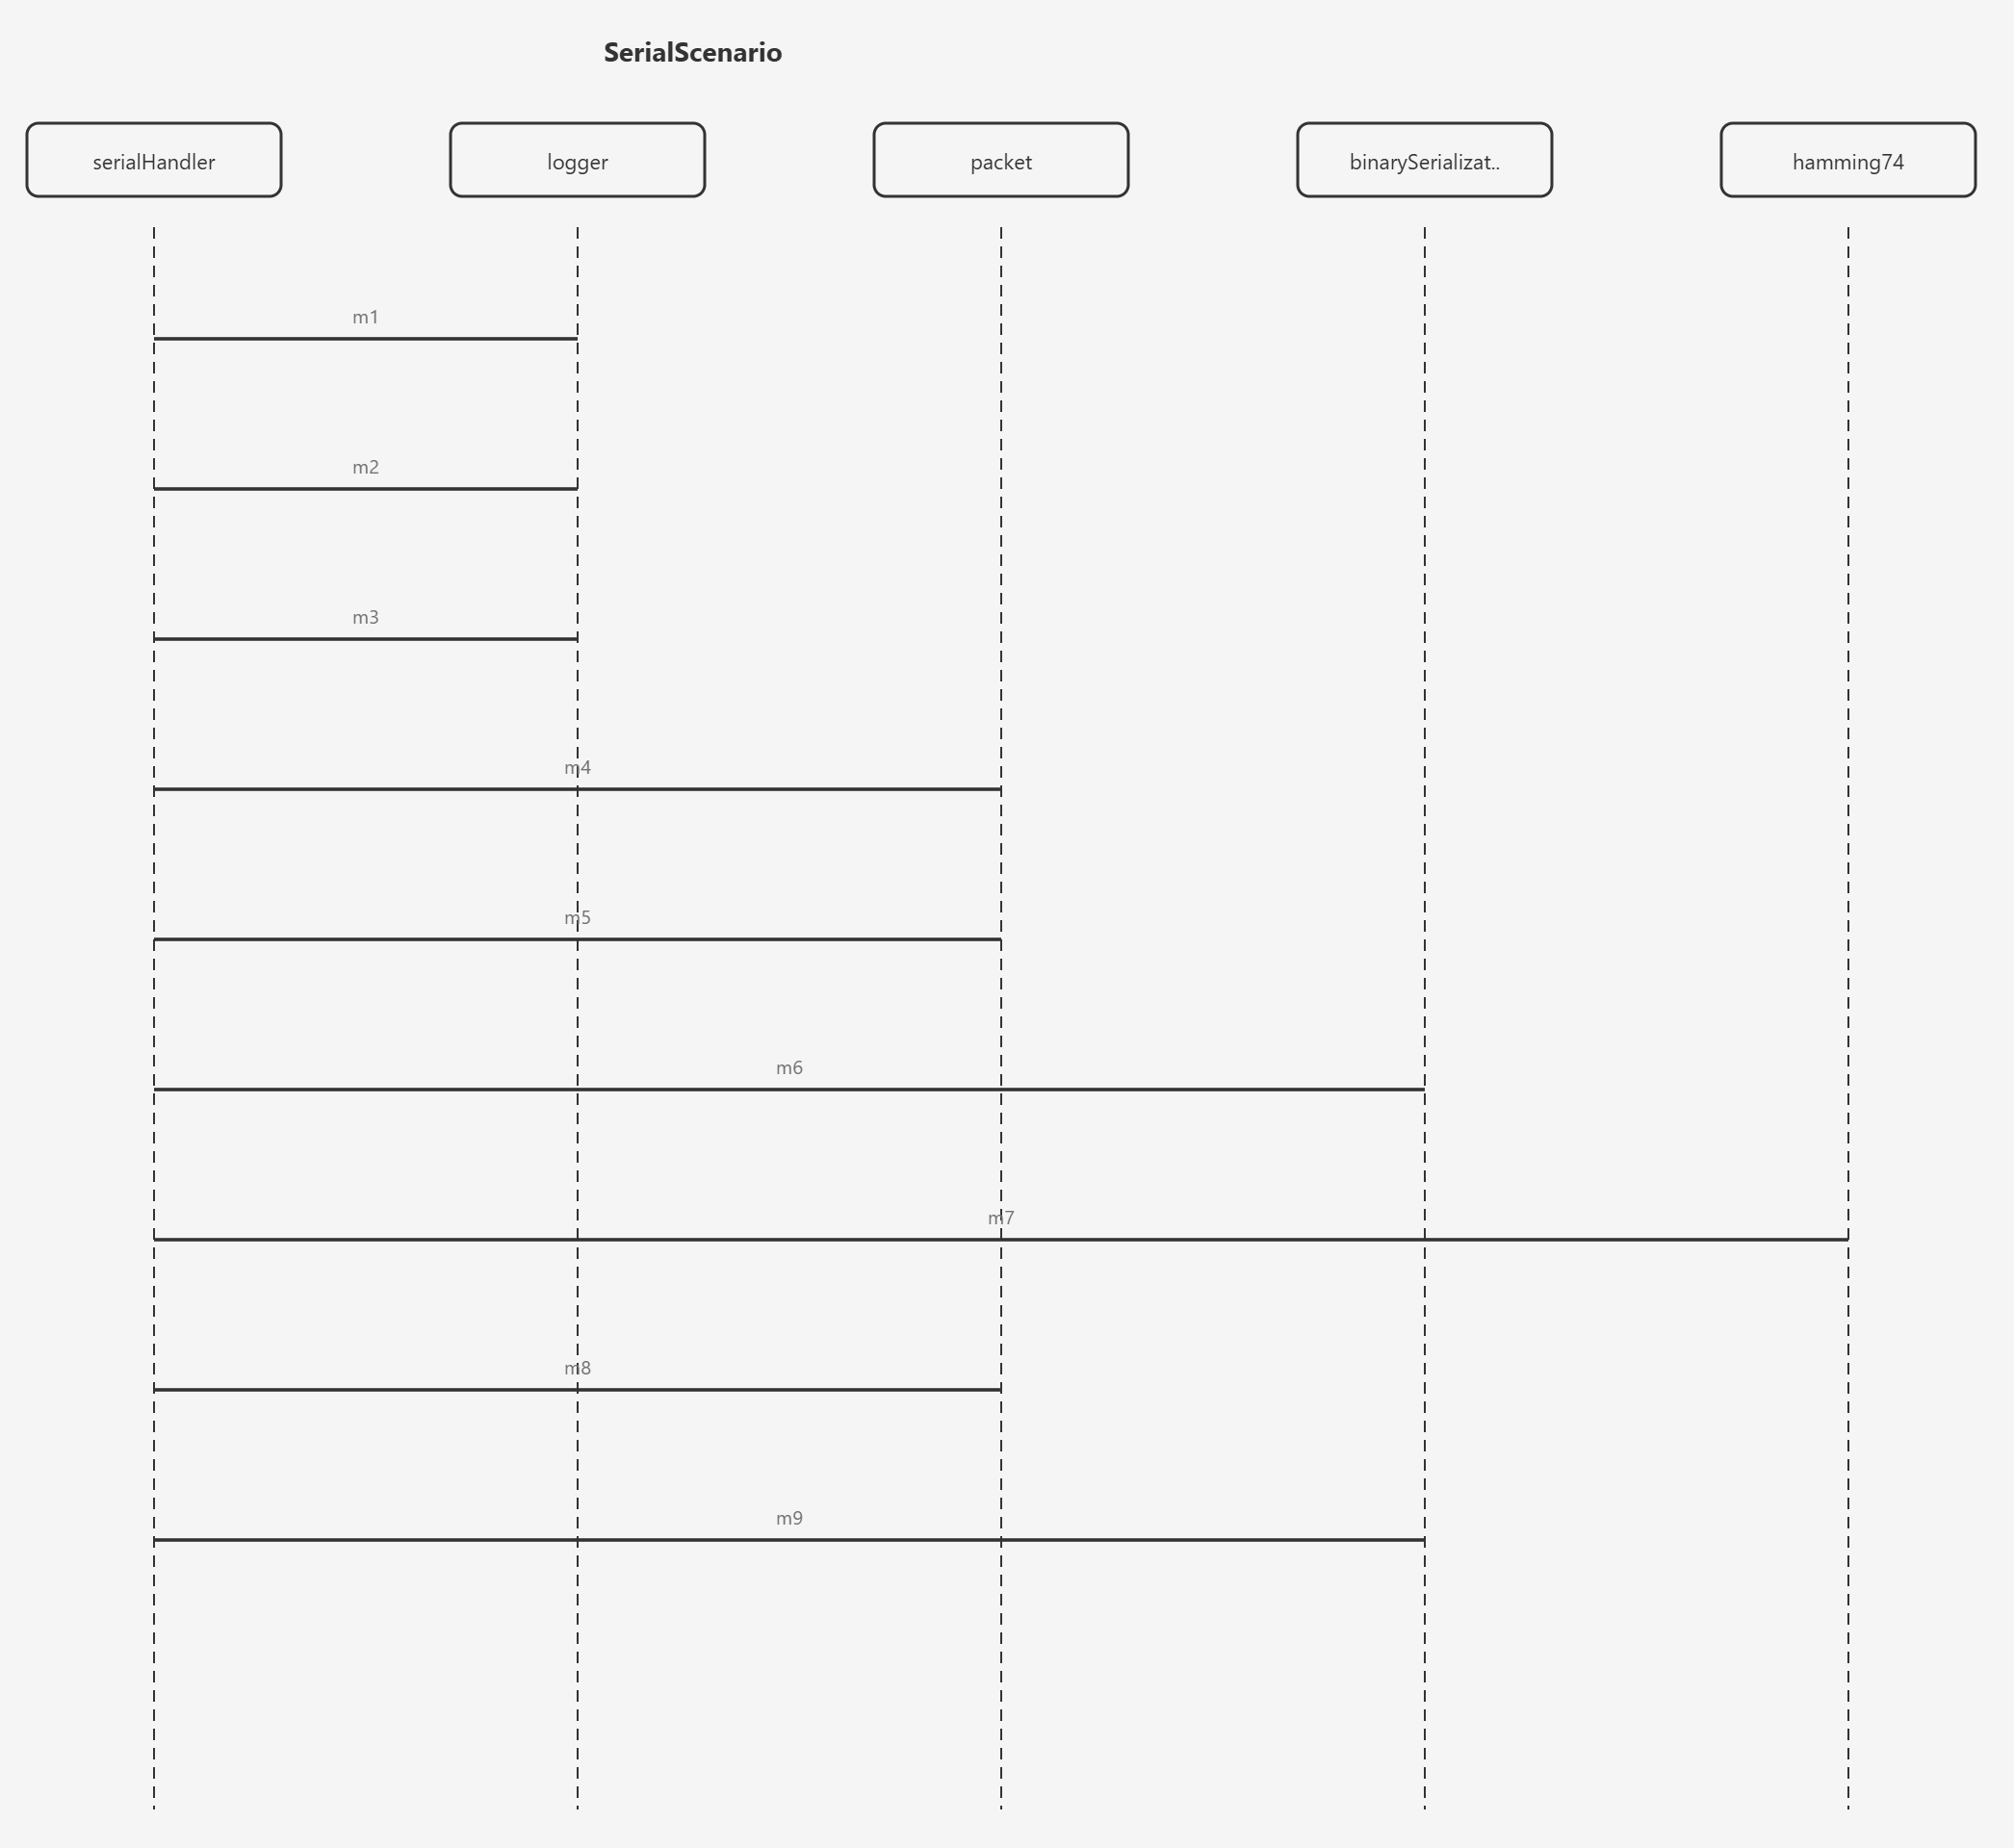
\includegraphics[width=0.85\textwidth]{figures/sysmlv2 diagrams/serialFlow.png}
  \caption{SysML v2 sequence diagram: Serial scenario showing data
    serialisation interactions (SerialHandler, Logger, Packet,
    BinarySerialization, Hamming74).}
  \label{fig:sysml-serial}
\end{figure}

\begin{figure}[H]
  \centering
  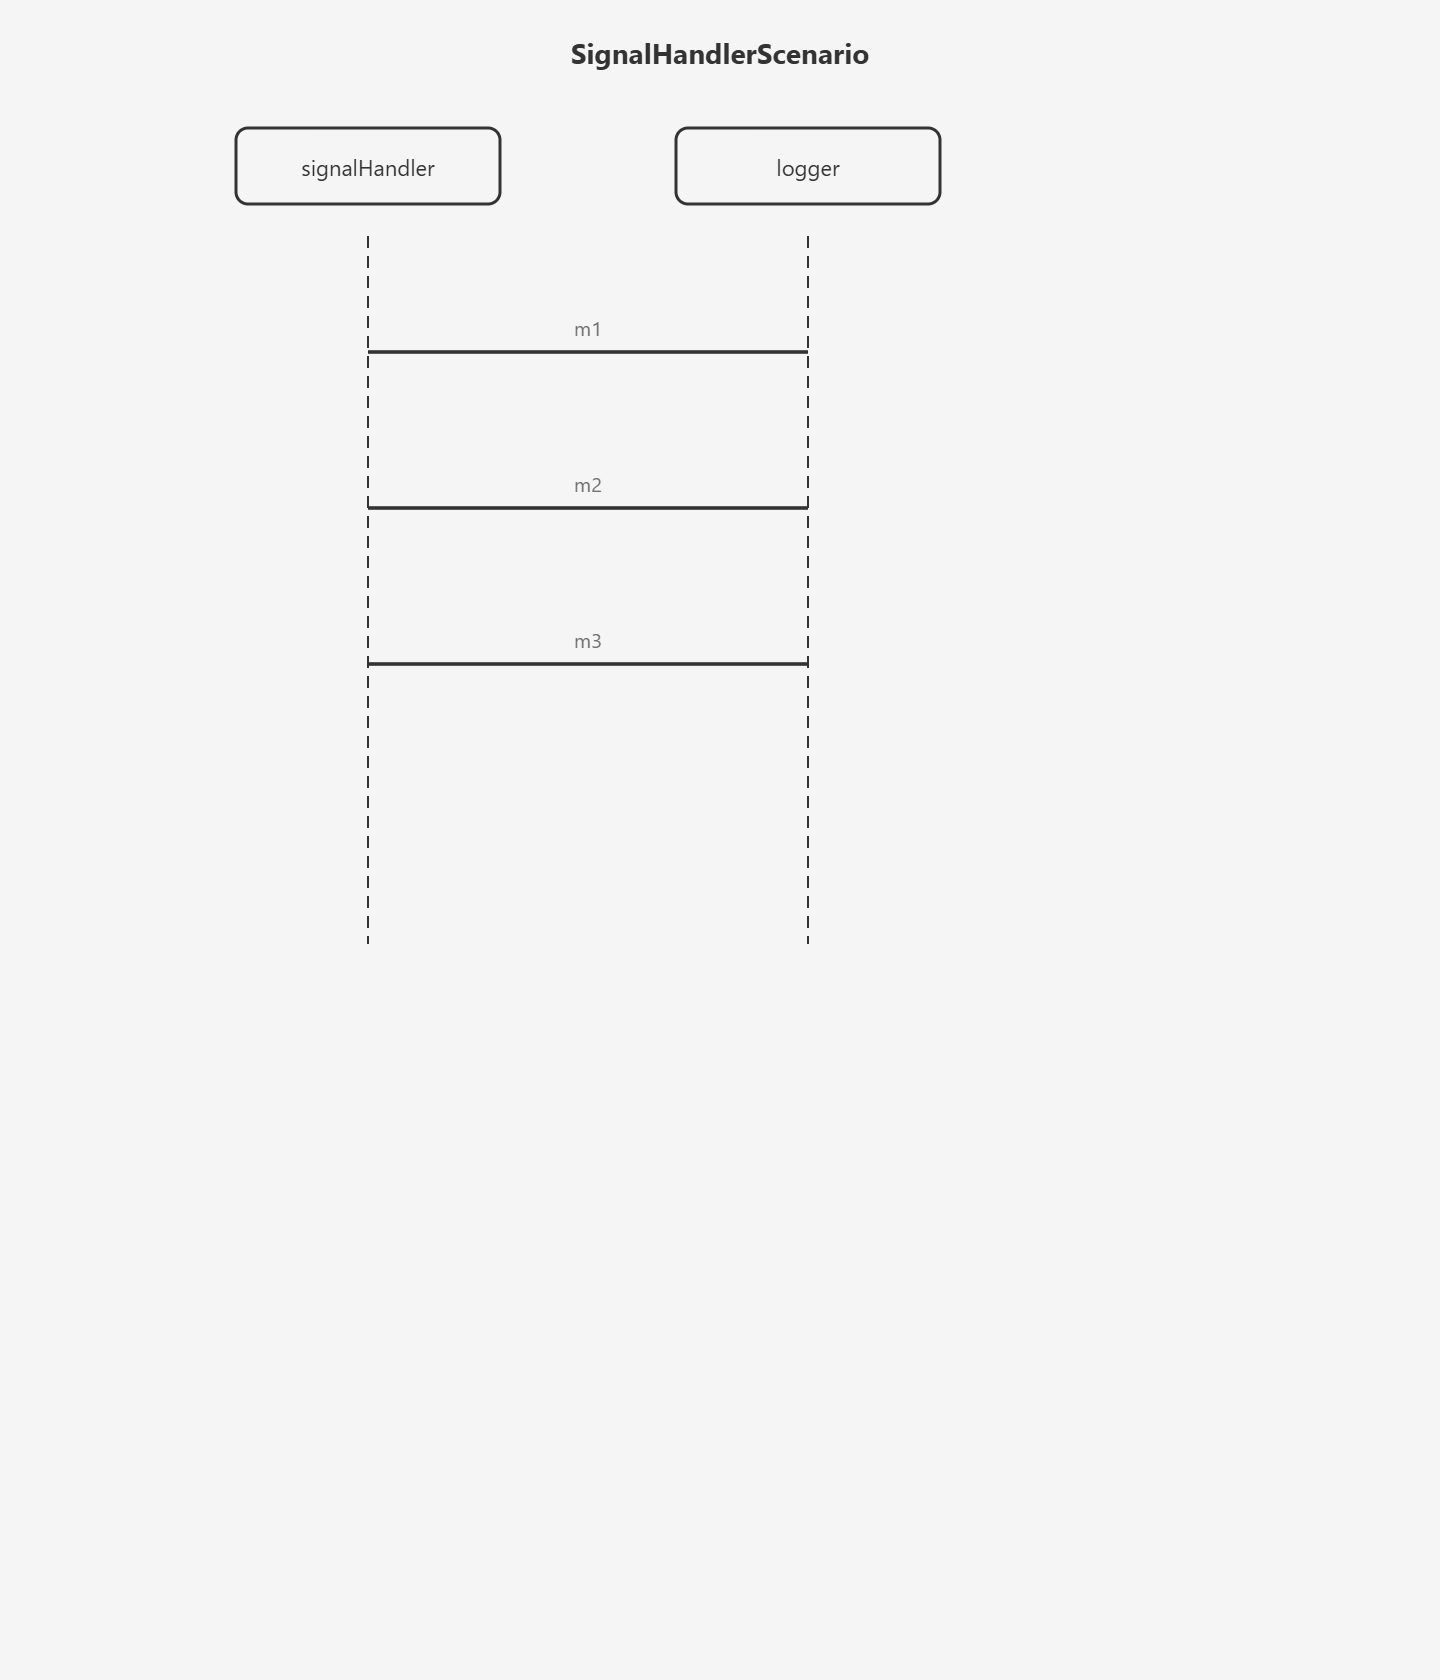
\includegraphics[width=0.7\textwidth]{figures/sysmlv2 diagrams/signalHandlerFlow.png}
  \caption{SysML v2 sequence diagram: Signal handler scenario showing the
    signal handling to logging interaction path (SignalHandler, Logger).}
  \label{fig:sysml-signalhandler}
\end{figure}

\begin{figure}[htbp]
  \centering
  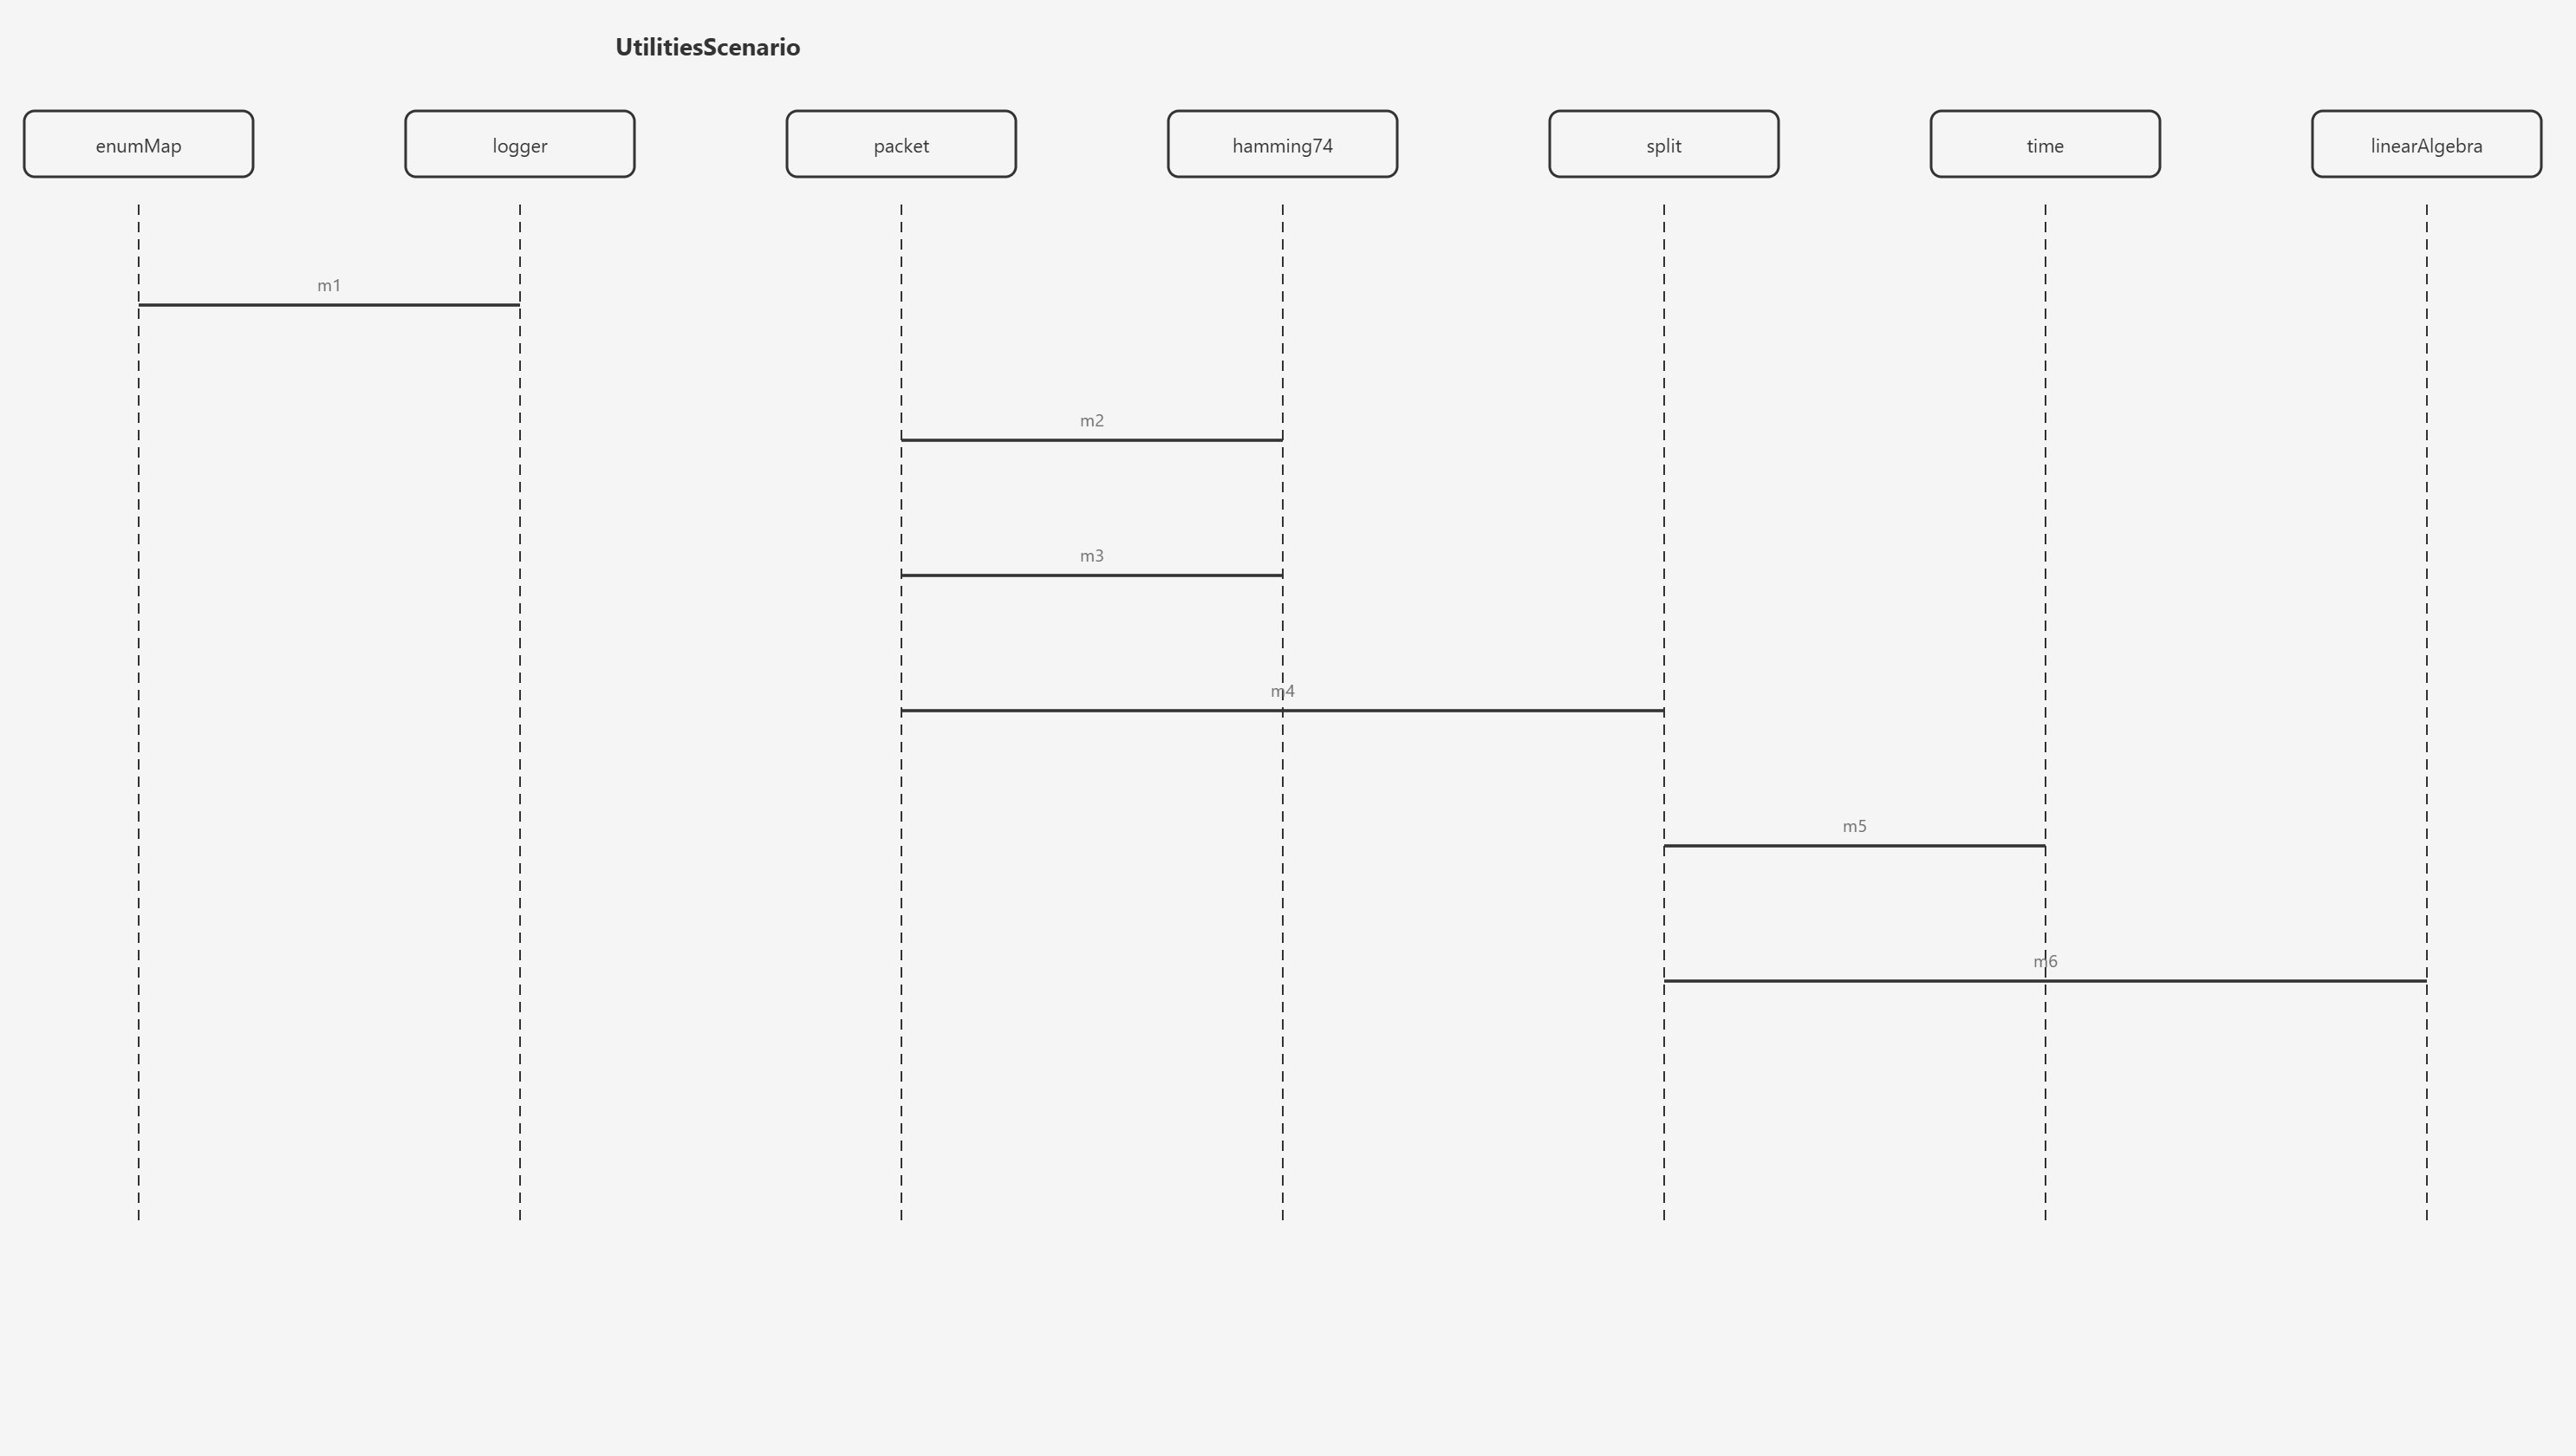
\includegraphics[width=0.9\textwidth]{figures/sysmlv2 diagrams/utilitiesFlow.png}
  \caption{SysML v2 sequence diagram: Utilities scenario showing cross-utility
    interactions (EnumMap, Logger, Packet, Hamming74, Split, Time,
    LinearAlgebra).}
  \label{fig:sysml-utilities}
\end{figure}

\begin{figure}[H]
  \centering
  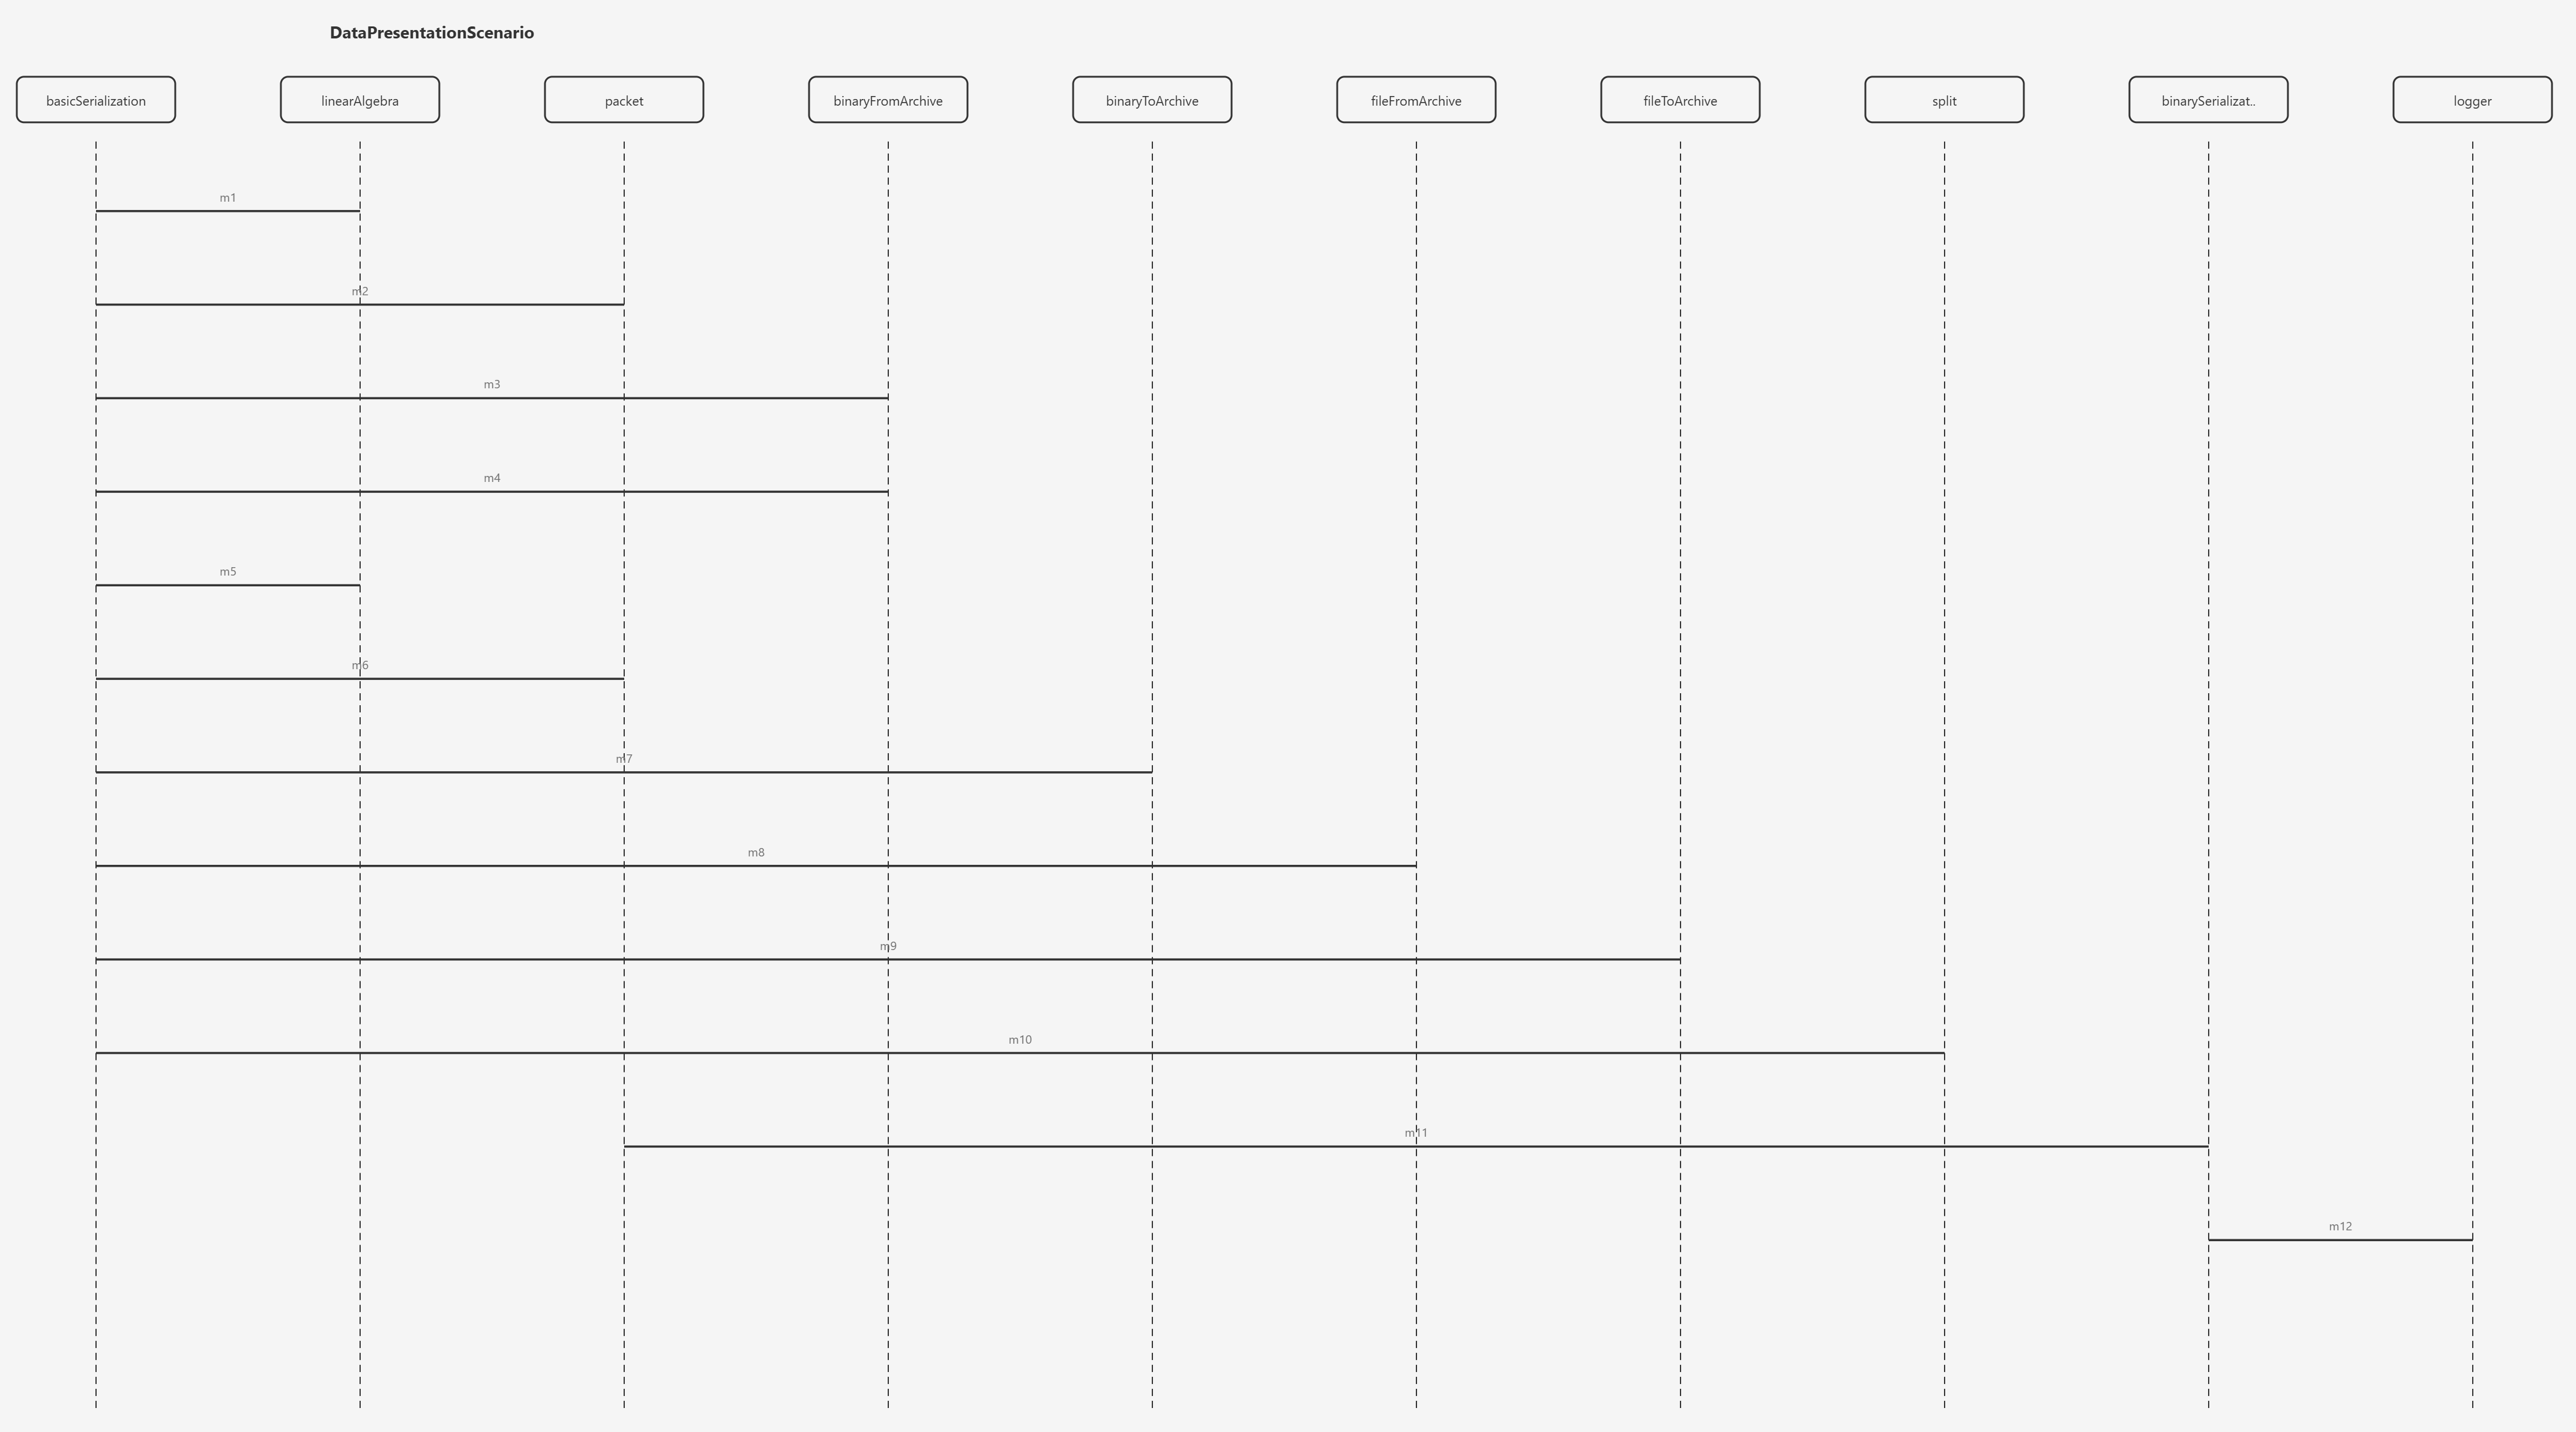
\includegraphics[width=0.85\textwidth]{figures/sysmlv2 diagrams/dataPresentationFlow.png}
  \caption{SysML v2 sequence diagram: Data presentation scenario showing
    Hamming74 encoding/decoding and packet-level interactions.}
  \label{fig:sysml-datapresentation}
\end{figure}

\begin{figure}[H]
  \centering
  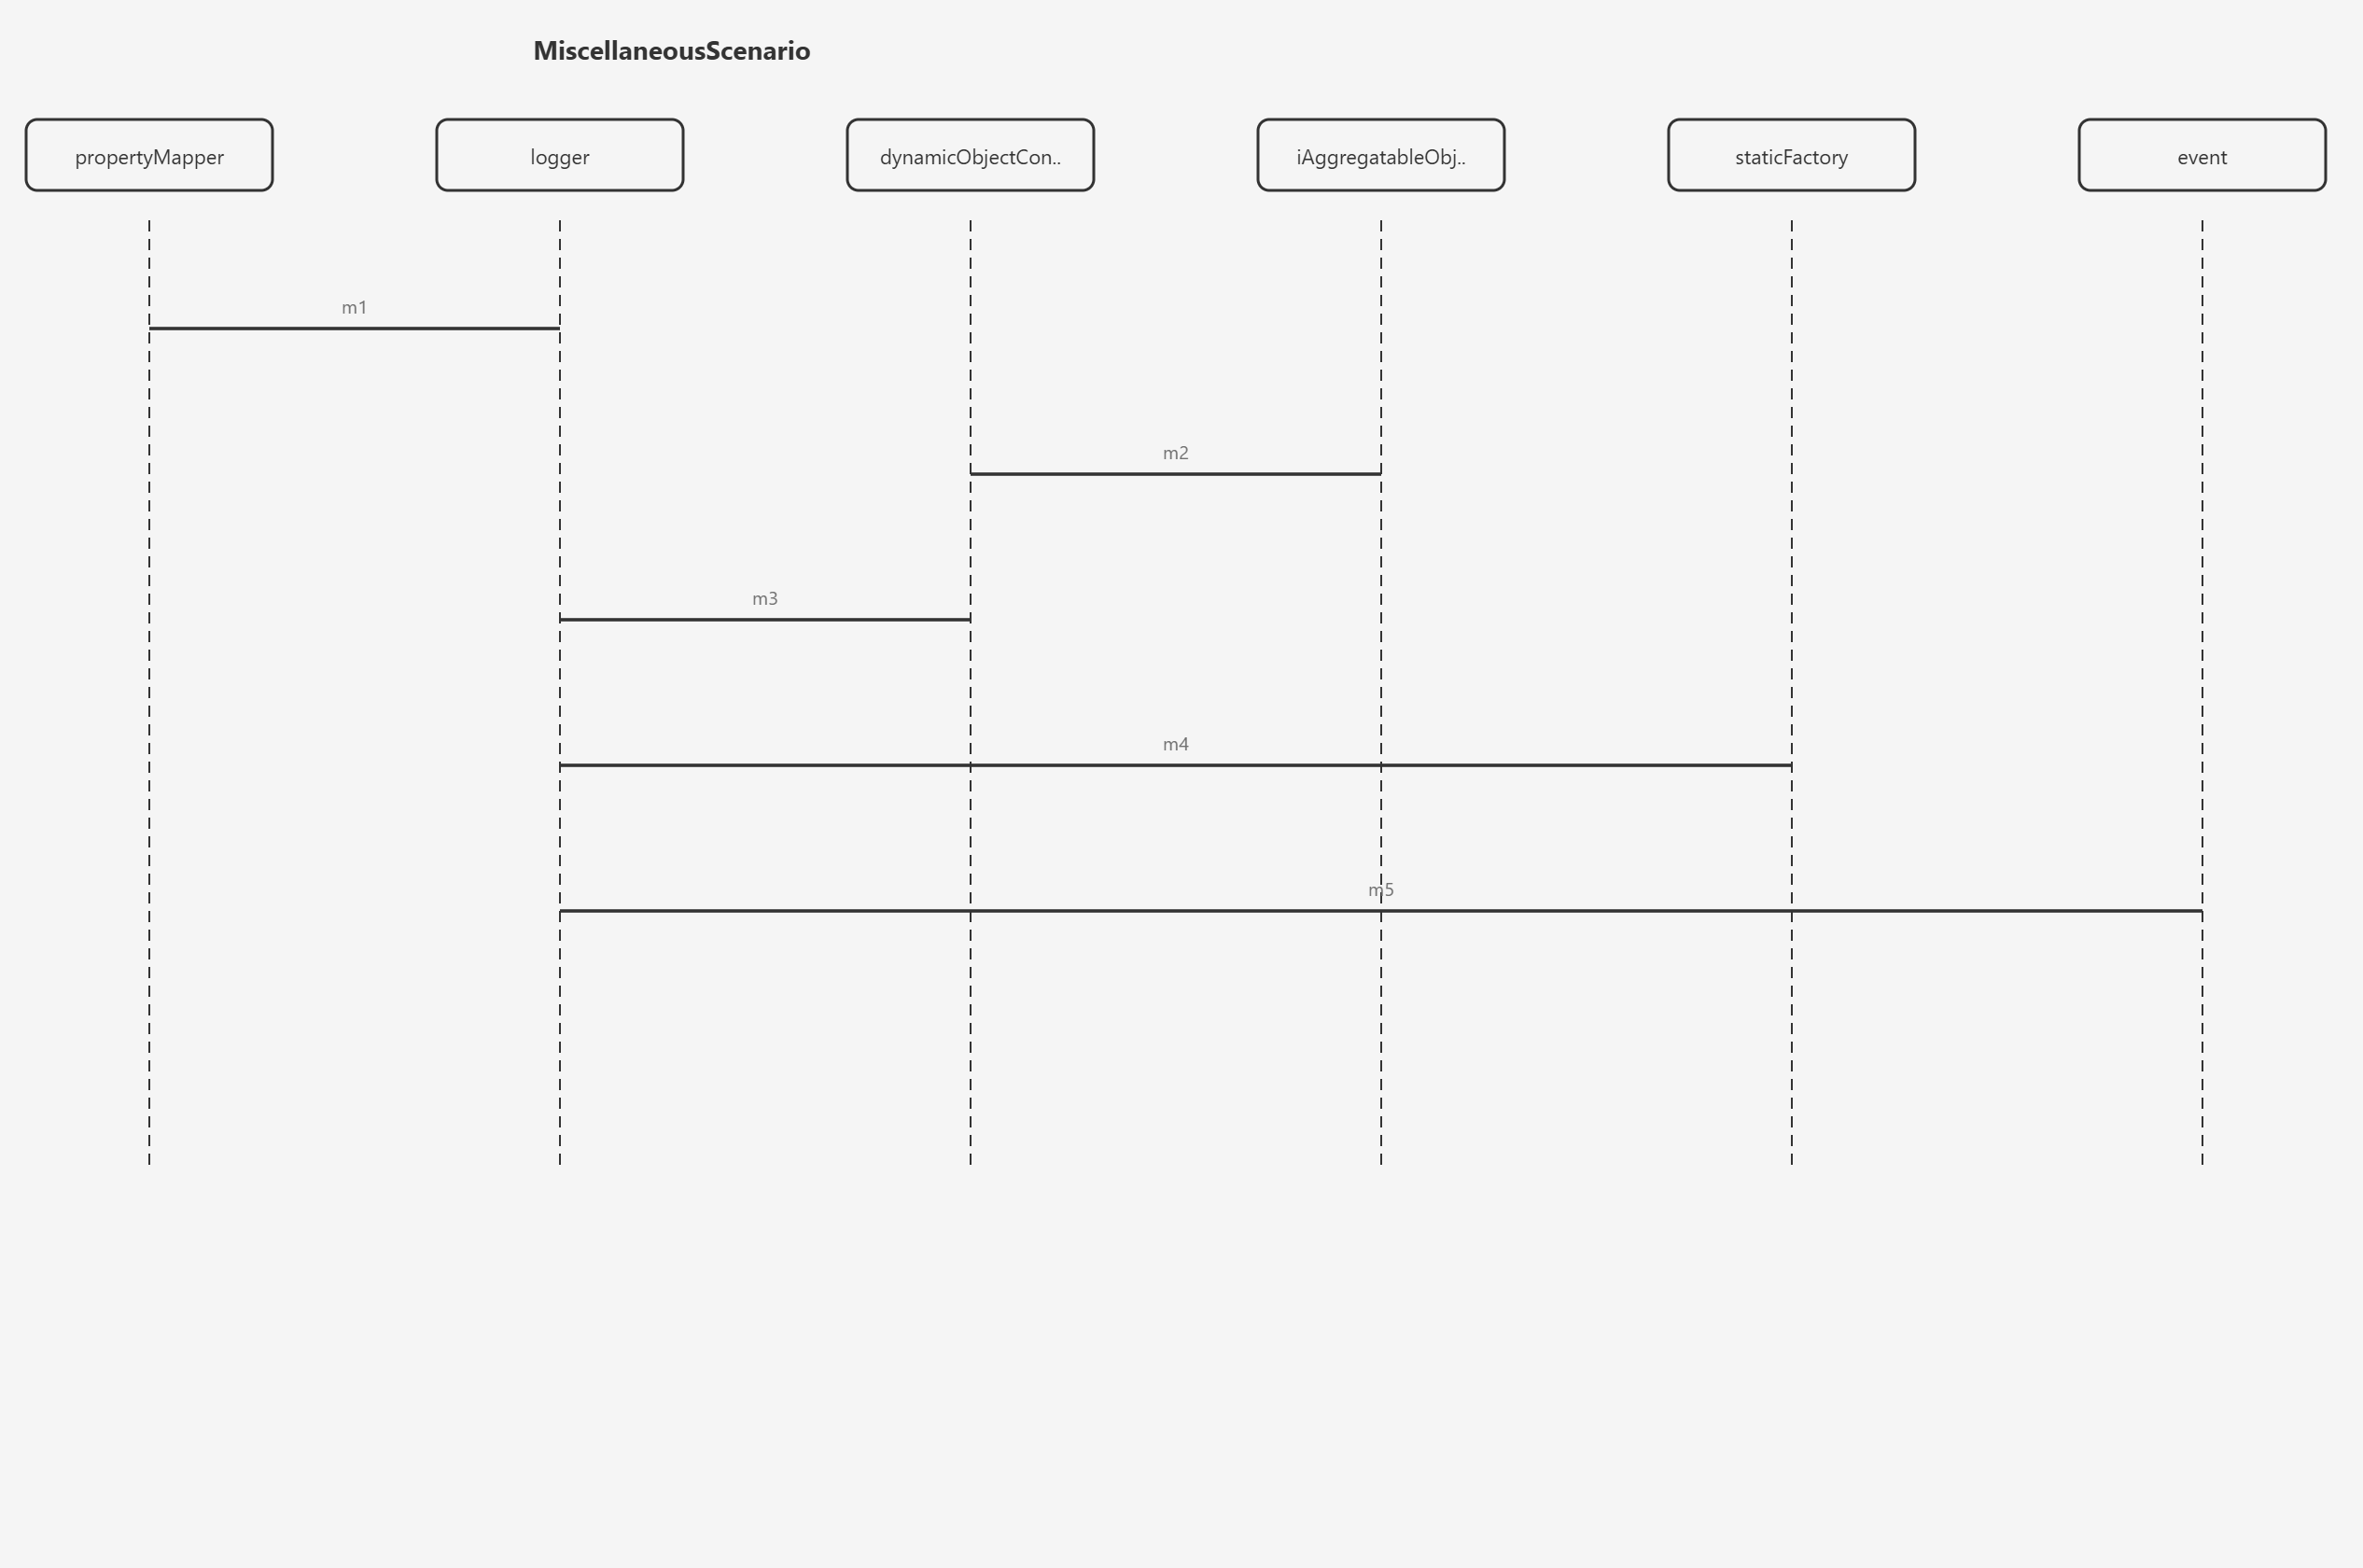
\includegraphics[width=0.85\textwidth]{figures/sysmlv2 diagrams/miscellaneousFlow.png}
  \caption{SysML v2 sequence diagram: Miscellaneous scenario showing
    PropertyMapper, Logger, DynamicObjectContainer, IAggregatableObject,
    StaticFactory, and Event interactions.}
  \label{fig:sysml-misc}
\end{figure}

\begin{figure}[htbp]
  \centering
  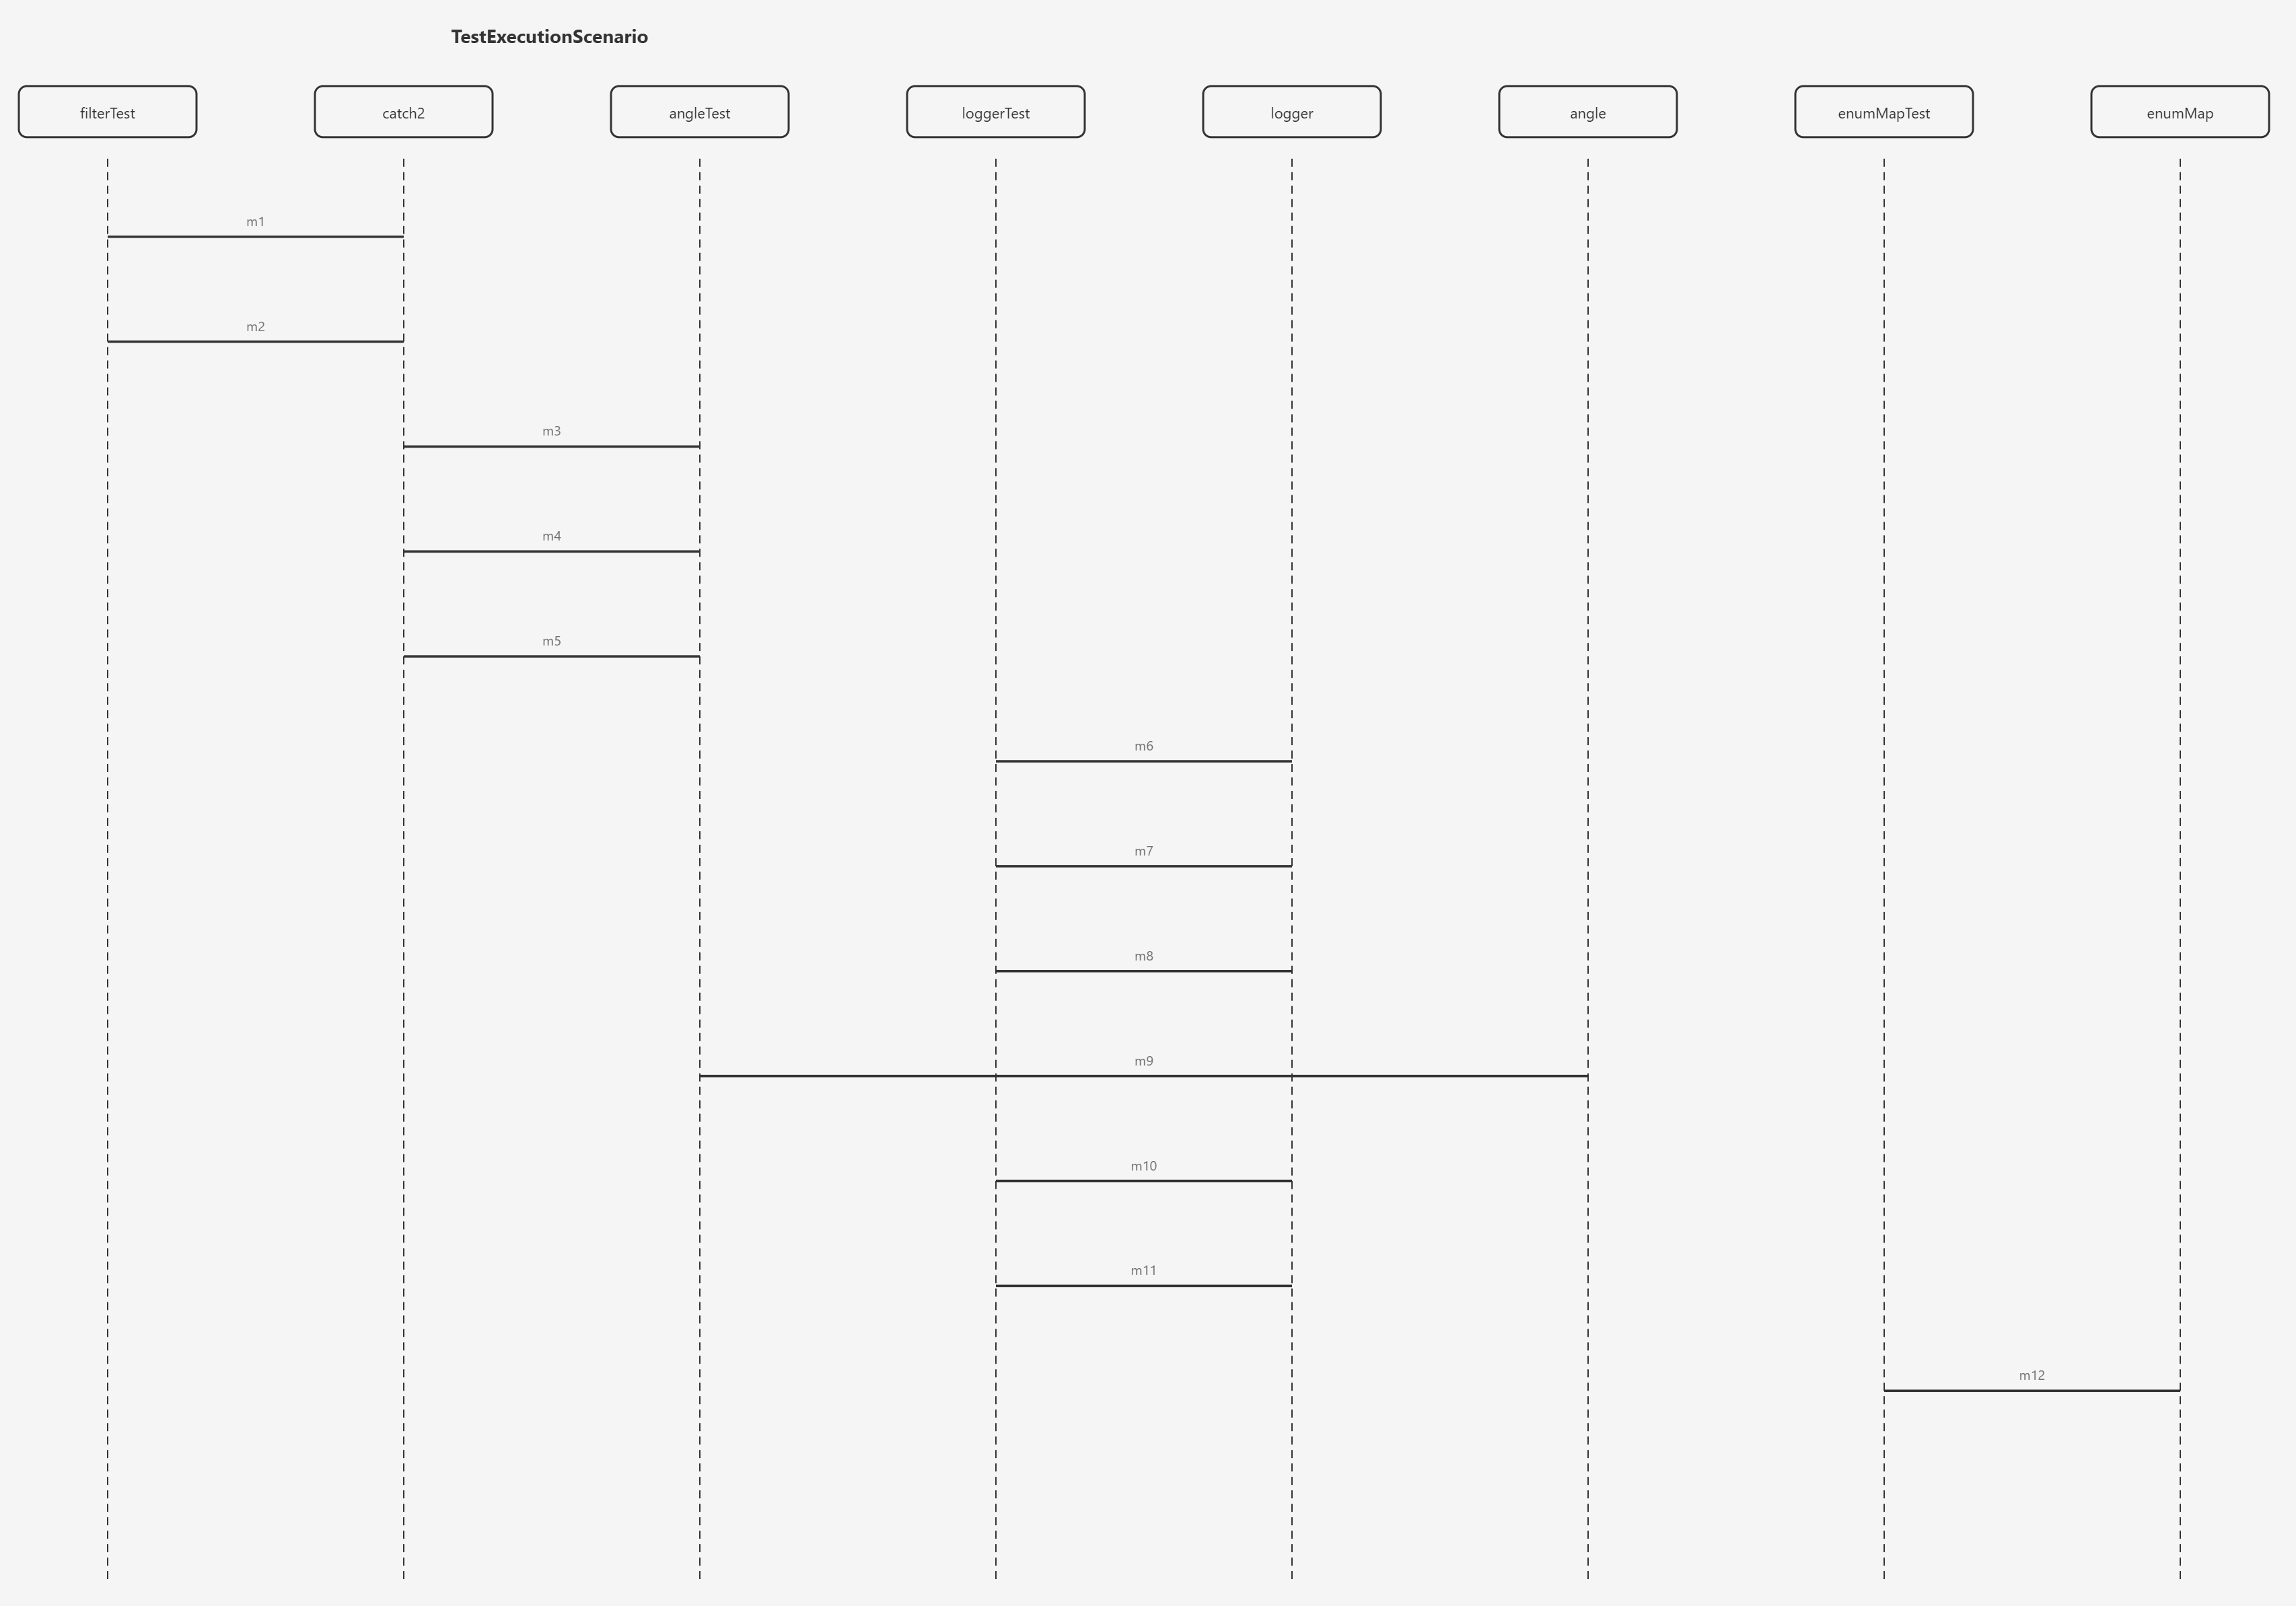
\includegraphics[width=0.9\textwidth]{figures/sysmlv2 diagrams/testExecutionFlow.png}
  \caption{SysML v2 sequence diagram: Test execution scenario showing
    the test framework interactions (FilterTest, Catch2, AngleTest,
    LoggerTest, Logger, Angle, EnumMapTest, EnumMap).}
  \label{fig:sysml-testexecution}
\end{figure}

\begin{figure}[H]
  \centering
  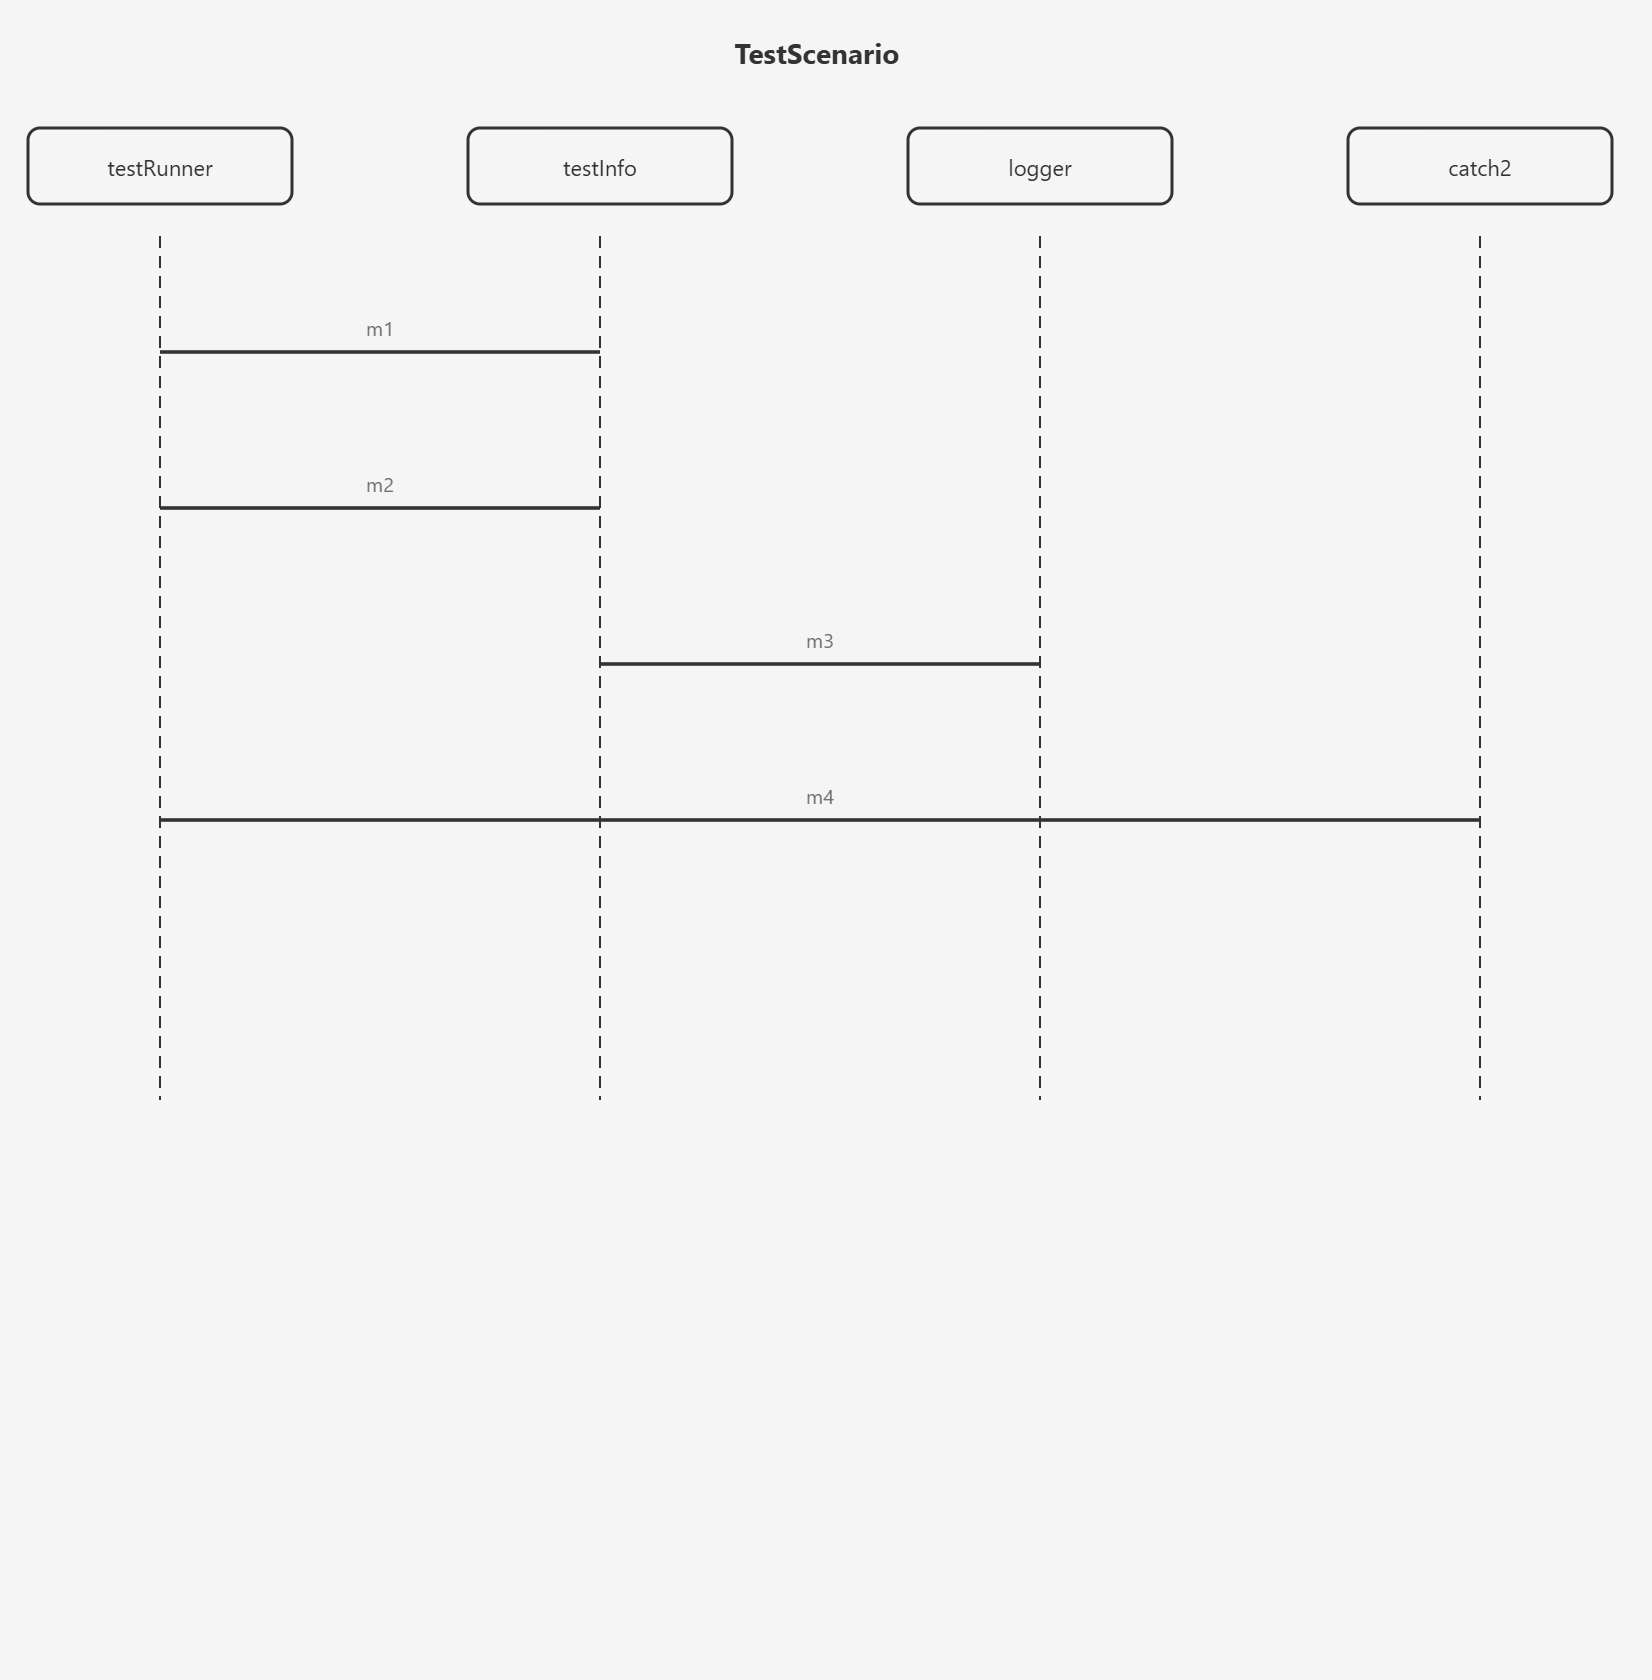
\includegraphics[width=0.7\textwidth]{figures/sysmlv2 diagrams/testFlow.png}
  \caption{SysML v2 sequence diagram: Test scenario showing test runner and
    test info interactions (TestRunner, TestInfo, Logger, Catch2).}
  \label{fig:sysml-test}
\end{figure}
